\chapter{Group theory}
The fundamental concept on which group theory is based on is, of course, the notion of group. Intuitively, one can think of a group as a collection of objects, that in principle can be of any kind, together with a particular internal binary operation that satisfies some requirements. Given the totally abstract nature of a group, this can be a really powerful tool with many applications. Nonetheless, a formal definition of a group is the following.
\begin{defn}[group]
    A group is a set of elements $G$ with an internal operation $\cdot : G \times G \to G$ that satisfies the following properties:
    \begin{enumerate}
        \item associativity, $(a \cdot b)\cdot c = a\cdot(b \cdot c)$, $\forall a,b,c\in G$;
        \item existence of unit element, $\exists e : a \cdot e = e \cdot a = a$, $\forall a\in G$;
        \item existence of inverse element, $\exists a^{-1} : a\cdot a^{-1} = a^{-1} \cdot a = e$, $\forall a \in G$.
    \end{enumerate}
\end{defn}
\begin{notz}
    A common notation that is used to indicate a group, which includes the set and the product, is $(G,\cdot)$. 
\end{notz}
\begin{defn}[Abelian group]
    A group $(G,\cdot)$ is Abelian if the commutative property is satisfied, so if
    \begin{equation}
        a \cdot b = b \cdot a,\quad \forall a,b \in G.
    \end{equation}
    If that's not the case, the group is non-Abelian.
\end{defn}
\begin{corl}[uniqueness of unit element]
    The unit element $e$ of a group $(G,\cdot)$ is unique.
\end{corl}
\begin{proof}
    Suppose for absurd that exists a second unit element $f \neq e \in G$. In that case, $f$ must satisfy the definition of unit element
    \begin{equation}
    \label{eq: unit element condition of f (proof of uniqueness)}
        f\cdot a = a \cdot f = a,\quad \forall a\in G.
    \end{equation}
    However, $e$ is by definition the unit element of $G$ so it must be true that
    \begin{equation}
    \label{eq: unit element condition of e (proof of uniqueness)}
        e \cdot a = a \cdot e = a,\quad \forall a\in G.
    \end{equation}
    Now if one applies the equation \eqref{eq: unit element condition of f (proof of uniqueness)} by imposing $a = e$, they will find that
    \begin{equation}
        e\cdot f = f \cdot e = e,
    \end{equation}
    but also if one impose $a = f$ in the relation \eqref{eq: unit element condition of f (proof of uniqueness)}, they will also find that
    \begin{equation}
        f \cdot e = e \cdot f = f.
    \end{equation}
    So it's immediate to see that it must be $e = f$, contradicting the initial hypothesis that $e \neq f$.
\end{proof}
\begin{corl}[uniqueness of inverse element]
    The inverse element $a^{-1}$ of a group $(G,\cdot)$ is unique.
\end{corl}
\begin{proof}
    The same reasoning followed in the proof of the uniqueness of the unit element is used here. So suppose that exists a second inverse element $b^{-1} \neq a^{-1} \in G$. The two inverse element must satisfy the defining condition by definition, so
    \begin{equation}
    \label{eq: inverse element conditions of a^-1 and b^-1 (proof of uniqueness)}
        \begin{cases}
            a^{-1} \cdot a = a \cdot a^{-1} = e \\
            b^{-1} \cdot a = a \cdot b^{-1} = e
        \end{cases}.
    \end{equation}
    If one multiplies the first equation of \eqref{eq: inverse element conditions of a^-1 and b^-1 (proof of uniqueness)} by $b^{-1}$, they will find that
    \begin{equation}
        (a^{-1} \cdot a) \cdot b^{-1}  = e \cdot b^{-1} = b^{-1},
    \end{equation}
    but if one use the associativity property of the group they will find that 
    \begin{equation}
        a^{-1} \cdot (a \cdot b^{-1}) = a^{-1} \cdot e = a^{-1}.
    \end{equation}
    So, again, it's immediate to see that it must be $a^{-1} = b^{-1}$, contradicting the initial hypothesis that $a^{-1} \neq b^{-1}$.
\end{proof}
Even though the conditions that define a group are apparently simple, they are quite constricting. One can in fact define a more general concept, the magma, as the following.
\begin{defn}[magma]
    A magma is a set of elements $M$ with an internal operation $\cdot : M \times M \to M$ that satisfies the following property
    \begin{equation}
        a \cdot b \in M,\quad \forall a,b\in M.
    \end{equation}
\end{defn}
If the operation of a magma satisfy only the property of associativity, then it becomes a semigroup
\begin{defn}[semigroup]
    A semigroup is a set of elements $S$ with an internal operation $\cdot : S \to S \times S$ that satisfies the property of associativity. 
\end{defn}
Also, if the operation of a semigroup satisfies the existence of the unit element, it becomes a monoid.
\begin{defn}[monoid]
    A monoid is a set of elements $M$ with an internal operation $\cdot : M \to M \times M$ that satisfies the property of associativity and of the existence of the unit element.
\end{defn}
An important aspect of a group is the amount of elements that contains, this is expressed by the order of a group.
\begin{defn}[order of a group]
    The order $|G|$ of a group $G$ coincides with its cardinality.
\end{defn}
Essentially, a group is said to be finite if the order $|G|$ is a number, but if the order $|G|$ is infinity one must make a distinction between countable and uncountable groups.  
\begin{defn}[countable group]
    A group $G$ is said to be countable if its order is a cardinal that is at the most the cardinality of natural numbers. If that's not the case the group is said to be uncountable.
\end{defn}
For a finite group, one can also define the order of an element which, despite the name, has nothing to do with the order of said group.
\begin{defn}[order of an element]
    Given a finite group $(G,\cdot)$, the order of an element $a \in G$ is the lowest $n \in \N$ such that 
    \begin{equation}
        a^n = a\cdot\underbrace{\cdots}_{n\,\mathrm{times}}\cdot a = e.
    \end{equation}
\end{defn}
The constraint that $G$ must be finite can be understood by considering the infinite group $(\Z,+)$ with unit element $e =0$ and an element $a \in \Z$, in this case there it does not exists an $n \in \N$ such that $a^n = 0$; obviously the equation is solved by $n = 0$ but, as said previously, $n$ must be a positive integer.
\begin{ex}
    An example of a infinite countable set is $\Z$, while a infinite uncountable set is $\R$.
\end{ex}
Consider now the set $G = \{e,a\}$ and the product $\cdot : G \to G \times G$ defined as
\begin{equation}
    \begin{cases}
        e \cdot e = e \\
        a \cdot e = a \\
        e \cdot a = a \\
        a \cdot a = a
    \end{cases}.
\end{equation}
The last relation is not obvious, it implies that $a$ is the inverse element of itself, so $a = a^{-1}$. If that was not the case and $a \cdot a^{-1} = e$, it would not work because one could derive 
\begin{align}
    a \cdot a \cdot a^{-1} &= a \cdot a^{-1} \notag \\
    a \cdot e &= e \\
    a &= e, \notag
\end{align}
which is a contradiction because it must be $a \neq e$ by definition of $G$. The group $(G,\cdot)$ defined as said it's named the ``cyclic group'' of order two $\Z_2$. Because of the fact that a group is an abstract concept, the elements of $\Z_2$ can be a lot of different things. For example, $\Z_2$ can be defined as $\Z_2 = (\{+1,-1\},\times)$ where the operation ``$\times$'' is the standard multiplication between numbers; instead it can be defined as $\Z_2 = (\{0,1\},+\,\mathrm{mod}\, 2)$ or, again, as $\Z_2 = (\{\mathrm{false},\mathrm{true}\},\mathrm{XOR})$, where ``$\mathrm{false}$'' and ``$\mathrm{true}$'' are boolean variables while $\mathrm{XOR}$ is the exclusive-or operation.
\begin{ex}
    Other example of groups can be: $(\Z,+)$ with $e = 0$ and $a^{-1} = -a$, which is also Abelian; or $(\R,+)$ with $e = 0$ and $a^{-1} = -a$; or $(\R,\times)$ with $e = 1$ and $a^{-1} = 1/a$; or $(\R^{n,n},+)$ which can be seen as $M$ copies of $(\R,+)$; or, again, $(\{ M\in \R^{n,n} : \det{M} \neq 0\}, \times_M)$, where $\times_M$ is the standard matrix multiplication, which is a really important group called the ``special linear group'' $GL(n,\R)$ that can also be seen as $n$ copies of $(\R,\times)$ and that is Abelian only if $n = 1$, otherwise it's non-Abelian. 
\end{ex}
For groups that do not have a large amount of elements one can define the ``Cayley table'' of the group. Because Cayley tables describe non-Abelian groups, in order to avoid confusion, the convention is that the factor that labels the row, termed ``nearer factor'' by Cayley, comes first, and that the factor that labels the column, or further factor, is second; a generic example of a Cayley table is given in table \ref{tab: generic Cayley table}.
\begin{table}[h]
    \centering
    \begin{tabular}{|c|cccc|}
        \hline
        & $b_1$ & $b_2$ & $\cdots$ & $b_{|G|}$ \\ \hline
        $a_1$ & $a_1b_1$ & $a_1b_2$ & $\cdots$ & $a_1b_{|G|}$ \\
        $a_2$ & $a_2b_1$ & $a_2b_2$ & $\cdots$ & $a_2b_{|G|}$ \\
        $\vdots$ & $\vdots$ & $\vdots$ & $\ddots$ & $\vdots$ \\
        $a_{|G|}$ & $a_{|G|}b_1$ & $a_{|G|}b_2$ & $\cdots$ & $a_{|G|}b_{|G|}$ \\ \hline
    \end{tabular}
    \caption{generic Cayley table of a group $G$ of order $|G|$.}
    \label{tab: generic Cayley table}
\end{table}

Another useful notion is the ``realisation'' of a group defined as the following.
\begin{defn}[realisation of a group]
    A realisation of a group $G$ is a map between any element $g\in G$ and a transformation $\rho(g)$ of some space $M$ in such a way that the group properties are preserved:
    \begin{enumerate}
        \item $\rho(e) = \mathrm{Id}$, the identity transformation;
        \item $\rho(g^{-1}) = [\rho(g)]^{-1}$;
        \item $\rho(g) \cdot \rho(h) = \rho(gh)$.
    \end{enumerate}
    The realisation can be:
    \begin{enumerate}
        \item ``faithful'' if the map is injective, so that
        \begin{equation}
            \rho(g) \neq \rho(h),\quad g \neq h;
        \end{equation}
        \item a ``representation of the group'' if $M$ is a vector space and every $\rho(g)$ is a linear transformation such that 
        \begin{equation}
            g \cdot v = \rho(g),\quad \forall g \in G,\,v\in M.
        \end{equation}
    \end{enumerate}
\end{defn}
One can also ``combine'' two groups into a third one by defining the ``direct product'' group.
\begin{defn}[direct product group]
    Given two groups $(G_1,\circ_1)$ and $(G_2,\circ_2)$ the set $G_1 \times G_2$ can be defined as the set of all the ordered couples $(g_1,g_2)$ with $g_1 \in G_1$ and $g_2 \in G_2$, together with an internal operation $* : G_1 \times G_1 \times G_2 \times G_2 \to G_1 \times G_2$ defined as
    \begin{equation}
        (g_1,g_2) * (g_1',g_2') := (g_1\circ_1 g_1',g_2\circ_2 g_2'),\quad g_1,g_1'\in G_1,g_2,g_2'\in G_2,
    \end{equation}
    which satisfies the properties of a group:
    \begin{enumerate}
        \item associativity;
        \item the existence of the unit element, $(e_1,e_2)$ with $e_1\in G_1, \,e_2\in G_2$;
        \item the existence of the inverse element, $(g_1,g_2)^{-1} := (g_1^{-1},g_2^{-1}),\,\forall g_1\in G_1,\,\forall g_2 \in G_2$.
    \end{enumerate}
\end{defn}
The dihedral group $D_n$ of order $n$ is defined as the set of transformations leaving the shape of a regular polygon with $n$ sides unchanged, in other words, it is the set of the $n$ rotations by $2\pi/n$ and of the $n$ reflections about axes that go through the vertices and midpoints of the sides. By this definition, $D_n$ has order $|D_n| = 2n$, and also it is Abelian only for $n = 1$, otherwise is non-Abelian. 

A really important group that emerges in a lot of places in Physics is the group defined as the set of linear transformations of an orthonormal frame of reference in $\R^2$. These transformations do not vary the angles between the vectors and their lengths, because of these properties there are not a lot of matrices that can represent these kind of transformations, so one has
\begin{align}
    M &= 
    \begin{pmatrix}
        \cos{\alpha} & \sin{\alpha} \\
        -\sin{\alpha} & \cos{\alpha}
    \end{pmatrix}
    ,\quad \det{M} = 1, \\
    M' &= 
    \begin{pmatrix}
        \cos{\alpha} & \sin{\alpha} \\
        \sin{\alpha} & -\cos{\alpha}
    \end{pmatrix}
    ,\quad \det{M'} = -1,
\end{align}
where $\alpha$ is the parameter of the transformation such that $\alpha \in [0,2\pi] \subseteq \R$. This group is the ``orthogonal group'' $O(2,\R)$ of order two, where the ``2'' in the argument symbolize that the elements of $O(2,\R)$ act on two dimensional objects, in this case two dimensional vectors. The orthogonal group can also be defined, like the name suggests, as the group of all two dimensional orthogonal matrices, so 
\begin{equation}
    O(2,\R) := (\{M \in \R^{2\times 2} : O^TO = OO^T = \MI\},\times_M).
\end{equation}
There are two subsets of $O(2,\R)$: the first is defined as all the orthogonal matrices with positive determinant, while the second as all the orthogonal matrices with negative determinant; these two subsets are not jointed so that $O(2,\R)$ is separable. The subset of all the matrices with positive determinant is called the ``special orthonormal group'' $SO(2,\R)$.

One can generalize the discussion to complex groups and speak about linear transformations in $\C^2$. In general, a matrix $A \in \C^2$ has the form
\begin{equation}
    A = 
    \begin{pmatrix}
        \alpha & \beta \\
        \gamma & \delta
    \end{pmatrix}
    ,\quad \alpha,\beta,\gamma,\delta \in \C.
\end{equation}
If one impose that $A$ is such that $A^\dg = A^{-1}$, supposing that $A$ is invertibile by requiring that $\det{A} \neq 0$, one has
\begin{equation}
    A^\dg = 
    \begin{pmatrix}
        \alpha^* & \gamma^* \\
        \beta^* & \delta^*
    \end{pmatrix}
    = 
    \begin{pmatrix}
        \delta & -\beta \\
        -\gamma & \alpha
    \end{pmatrix}
    = A^{-1}
\end{equation},
which implies that $\alpha^* = \delta$ and $\gamma^* = -\beta$. The general matrix $A$ then, imposing that $\det{A} = 1$, can be written as
\begin{equation}
\label{eq: element of SU(2,C)}
    A = 
    \begin{pmatrix}
        \alpha & \beta \\
        -\beta^* & \alpha^*
    \end{pmatrix},\quad \det{A} = 1,
\end{equation}
with determinant given by 
\begin{equation}
\label{eq: group condition of SU(2,C) in terms of matrix entries}
    \alpha\delta - \beta\gamma = |a|^2 + |b|^2 = 1.
\end{equation}
The group defined as the set of elements like the one in equation \eqref{eq: element of SU(2,C)} is called the ``special unit group'' $SU(2,\C)$. Now, if one writes the entries $\alpha$ and $\beta$ by explicitly showing their real and imaginary parts as
\begin{equation}
    \alpha = a_0 + ia_3,\quad \beta = a_2 + ia_1,\quad a_0,a_1,a_2,a_3 \in \R,
\end{equation}
the condition \eqref{eq: group condition of SU(2,C) in terms of matrix entries} can be written as 
\begin{equation}
\label{eq: group condition of SU(2,C) in terms of the real and imaginary parts of matrix entries}
    a_0^2 + a_1^2 + a_2^2 + a_3^2 = 1.
\end{equation}
It is immediate to notice that the condition found in \eqref{eq: group condition of SU(2,C) in terms of the real and imaginary parts of matrix entries} is the same as the one that describes a surface of a unit sphere in $\R^4$, this is noted as $S^3 \subset \R^4$. The peculiar choice made when naming the real and imaginary parts of $\alpha$ and $\beta$ is not by chance, it is justified by the fact that $A$ can be written as
\begin{equation}
    A = 
    \begin{pmatrix}
        a_0 + ia_3 & a_2 + ia_1 \\
        -a_2 + ia_1 & a_0 - ia_3
    \end{pmatrix}
    = a_0\MI + i\va \cdot \vsigma, 
\end{equation}
where $\va$ is a three dimensional vector $\va = (a_1,a_2,a_3)$ and $\vsigma$ is defined through the Pauli matrices $\sigma_i$ as $\vsigma = (\sigma_1,\sigma_2,\sigma_3)$. Now one can show that $A^{-1} = A^\dg$; in fact $A^\dg$ is just 
\begin{equation}
    A^\dg = (a_0\MI + i\va \cdot \vsigma)^\dg = a_0\MI - i\va \cdot \vsigma = 
    \begin{pmatrix}
        a_0 - ia_3 & -a_2 - ia_1 \\
        a_2 - ia_1 & a_0 + ia_3
    \end{pmatrix},
\end{equation}
that, is one does the calculation, satisfies the property $AA^\dg = \MI$, for every $A \in SU(2,\C)$. The calculation can be done by knowing the relations 
\begin{align}
    \acomm{\sigma^i}{\sigma^j} &= \sigma^i\sigma^j + \sigma^j\sigma^i = 2\delta^{ij}\MI, \\
    \comm{\sigma^i}{\sigma^j} &= \sigma^i\sigma^j - \sigma^j\sigma^i = 2i\epsilon^{ijk}\sigma^k,
\end{align}
that can be used to see that
\begin{equation}
    \begin{split}
        AA^\dg &= (a_0\MI + i\va \cdot \vsigma)(a_0\MI - i\va \cdot \vsigma) \\
        &= a_0^2\MI - ia_0\va \cdot \vsigma + ia_0\va \cdot \vsigma + a_ia_j\sigma_i\sigma_j \\
        &= a_0^2\MI + a_ia_j\frac{1}{2}(\acomm{\sigma^i}{\sigma^j} + \comm{\sigma^i}{\sigma^j}) \\
        &= a_0^2\MI + \frac{1}{2}a_ia_j\acomm{\sigma^i}{\sigma^j} \\
        &= (a_0^2 + a_k^2)\MI \\
        &= (a_0^2 + a_1^2 + a_2^2 + a_3^2)\MI \\
        &= \MI.
    \end{split}
\end{equation}
There is yet another way to see this. Consider the expression
\begin{equation}
    \exp{(i\phi\hatv\cdot\vsigma)} = \sum_{n = 0}^\infty \frac{(i\phi \hatv\cdot\vsigma)^n}{n!},
\end{equation}
which is legitimate because the arguments are matrices. Now, that is also equal to 
\begin{equation}
    \exp{(i\phi\hatv\cdot\vsigma)} = (\cos{\phi})\MI + i(\sin{\phi})\hatv\cdot\vsigma \equiv a_0\MI + i\va\cdot\vsigma,
\end{equation}
that also satisfies the condition \eqref{eq: group condition of SU(2,C) in terms of the real and imaginary parts of matrix entries}
\begin{equation}
    |\cos{\phi}|^2 + |\sin{(\phi)}\hatv|^2 = |\cos{\phi}|^2 + |\sin{\phi}|^2 = 1,\quad |\hatv|^2 = 1,\,\phi\in[0,\pi].
\end{equation}
The discussion can now continue by defining what is a subgroup and some of its properties. 
\begin{defn}[subgroup]
    Given a group $(G,\cdot)$ and a set $H \subseteq G$, if the object $(H,\cdot)$ is also a group than $H$ is a subgroup of $G$, indicated as $H \le G$.
\end{defn}
\begin{defn}[trivial subgroup]
    $(H,\cdot)$ is a trivial subgroup of $(G,\cdot)$ if $H \equiv G$ or if $H = \{e\}$. 
\end{defn} 
By this definition, if a subgroup $H \le G$ is not trivial then $H$ is said to be a ``proper subgroup''. Also, if $H \le G$ then $H$ must contain the unit element.
\begin{defn}[normal subgroup]
    A subgroup $(H,\cdot)$ of a group $(G,\cdot)$ is said to be a normal subgroup if it true that
    \begin{equation}
        ghg^{-1} \in H,\quad \forall g\in G,\, \forall h \in H.
    \end{equation}
\end{defn}
An interesting fact is that a subgroup $(H,\cdot)$ of an Abelian group $(G,\cdot)$ is always a normal subgroup. 
\begin{defn}[semi-simple group]
    A group $(G,\cdot)$ with no proper normal Abelian subgroup is said to be a semi-simple group.
\end{defn}
\begin{defn}[simple group]
    A group $(G,\cdot)$ with no proper normal subgroup is said to be a simple group.
\end{defn}
By these definitions one can tell that a semi-simple group is not necessarily simple, but a simple group is always semi-simple. 

It is now interesting to study the mappings between different groups through the notions of homomorphisms and isomorphisms. Before that, it is useful to introduce some useful definitions. 
\begin{defn}[equivalence relation]
    Let $X$ be a set and $\diamond$ a binary operation defined in $X$, the operation $\diamond$ is an equivalence relation if it is:
    \begin{enumerate}
        \item reflective, so that $\forall a \in X,\, a \diamond a$ is true;
        \item symmetric, so that $\forall a,b \in X : (a \diamond b)\Rightarrow(b \diamond a)$;
        \item transitive, so that $\forall a,b,c \in X : ((a \diamond c)\,\mathrm{and}\,(b \diamond c))\Rightarrow(a \diamond c)$.
    \end{enumerate}
\end{defn}
When one has an equivalence relation then they can use it to define equivalence classes.
\begin{defn}[equivalence class]
    Given a set $X$ and an equivalence relation $\diamond$ among its elements, the equivalence class of a generic element $a \in X$ is the subset of $X$ containing all elements $x$ such that $x \diamond a$ holds and it is denoted as $[a]$.
\end{defn}
The equivalence classes of a set $X$ do not intersect with each other and they are not empty, in fact they are denoted with $[x]$, where $x$ symbolizes all the elements that are contained by the equivalence class. Furthermore, the set of equivalence classes of a set $X$ is called the ``quotient space'' of said set and it is denoted by $X/\diamond$. Now, to define the concepts of homomorphism and isomorphism is necessary to introduce the notion of a injective and surjective function. Given two arbitrary, non-empty sets $X$ and $Y$, let $Map(X,Y)$ denote the set of functions, or mappings, from $X$ to $Y$ as
\begin{equation}
\label{eq: definition of Map(X,Y)}
    Map(X,Y) := \{f : X \to Y : \forall x \in X : \exists! f(x) \in Y\}.
\end{equation}
Within the set $Map(X,Y)$ there exist special types of functions.
\begin{defn}[injective function]
    A function $f : X \to Y$ is injective if it is true that
    \begin{equation}
        \forall x,a \in X,\, x \neq a \Rightarrow f(x) \neq f(a).
    \end{equation}
\end{defn}
\begin{defn}[surjective function]
    A function $f : X \to Y$ is surjective if it is true that 
    \begin{equation}
        \forall y \in Y,\, \exists x \in X : f(x) = y.
    \end{equation}
\end{defn}
\begin{defn}[bijective function]
    A function $f : X \to Y$ is bijective if it is both injective and surjective, equivalently if it is true that
    \begin{equation}
        \exists f^{-1} : Y \to X : f^{-1}(f(x)) = x,\,\forall x \in X. 
    \end{equation}
\end{defn}
Now homomorphisms and isomorphisms can be defined.
\begin{defn}[homomorphism]
    Given two groups $(G,\cdot)$ and $(H,*)$, a function $f : (G,\cdot) \to (H,*)$ is a homomorphism if
    \begin{equation}
        \forall g_1,g_2 \in G, f(g_1 \cdot g_2) = f(g_1) * f(g_2).
    \end{equation}
\end{defn}
\begin{defn}[isomorphism]
    An isomorphism is a bijective homomorphism.
\end{defn}

\section{Smallest finite groups}
Finite groups have several applications in Physics such as in classical mechanics where they can be used to reduce the number of relevant degrees of freedom in system with certain symmetries, as well in many areas of modern Physics. For certain sufficiently small finite sets, the requirements that a binary operation on the set of elements has to satisfy in order to be a group multiplication, are so constraining that they uniquely define the group. In the following there is a list of all the groups with order less than six; one has to notice that since a group must at least contain the unit element, the minimum order of a group is one.

\subsubsection{Order one}
The smallest group of order one is the ``trivial group'' $G = \{e\}$ containing only the unit element which, by definition, is the inverse of itself. 

\subsubsection{Order two}
A general group of order two is $G = \{e,a\}$ with $e \neq a$. The definition of the unit element implies that $e \cdot e = e$ and $e \cdot a = a$, so the only remaining operation that is unknown is $a \cdot a$ whose result, in order to be an element of the group itself, must be $e$ or $a$. However, this is a problem that has already been treated when talking about the cyclic group $\Z_2$ of order two. In fact, as said previously, the only possibility is $a \cdot a = e$, otherwise one will get a contradiction where $a = e$, which is obviously not the case since by definition of $G$ consider $a \neq e$. Accordingly, the Cayley table of the group of order two is uniquely fixed to be the one in \ref{tab: Z2 Cayley table}, and because of that $\Z_2$ is the only group of order two.
\begin{table}[h]
    \centering
    \begin{tabular}{|c|cc|}
        \hline
        & $e$ & $a$ \\ \hline
        $e$ & $e$ & $a$ \\
        $a$ & $a$ & $e$ \\ \hline
    \end{tabular}
    \caption{Cayley table of $\Z_2$ group.}
    \label{tab: Z2 Cayley table}
\end{table}

\subsubsection{Order three}
A general group of order three is $G = \{e,a,b\}$ with $e \neq a \neq b$. It turns out, again, that there is only one group of order three. The group can be determined by working out its Cayley table. To complete it, one need to determine first $a \cdot b$. To do that one can suppose that $a \cdot b = b$, in this case one gets 
\begin{equation}
    \begin{split}
        a \cdot b &= b \\
        (a\cdot b)\cdot b^{-1} &= b\cdot b^{-1} \\
        a \cdot (b \cdot b^{-1}) &= e \\
        a &= e,
    \end{split}
\end{equation}
which is a contradiction by definition of $G$ since $a \neq e$. So, another option is to suppose that $a \cdot b = a$, in this case one gets
\begin{equation}
    \begin{split}
        a \cdot b &= a \\
        a^{-1} \cdot (a \cdot b) &= a^{-1} \cdot a \\
        b &= e,
    \end{split}
\end{equation}
which is again a contradiction since $b \neq e$ by definition. Therefore, the only option acceptable is that $a \cdot b = a$. Similarly, for $a \cdot a \equiv a^2$ one can suppose that $a^2 = a$, but again gets
\begin{equation}
    \begin{split}
        a^2 &= a \\
        a^2 \cdot a^{-1} &= a \cdot a^{-1} \\
        a \cdot e &= e \\
        a &= e,
    \end{split} 
\end{equation}
which is another contradiction, and if one suppose that $a^2 = e$ then they get
\begin{equation}
    \begin{split}
        a^2 &= e \\
        a^2 \cdot b &= e \cdot b \\
        a \cdot (a\cdot b) &= b \\
        a &= b,
    \end{split}
\end{equation}
where it was used the relation $a\cdot b = e$ determined before, however the result is again a contradiction. Therefore, the only option is that $a^2 = b$, similarly one can show that $b^2 = a$. Hence, the complete Cayley table for the group of order three is unique, like the order two case, resulting in only one existing group of order three, as shown in \ref{tab: Z3 Cayley table}.
\begin{table}[h]
    \centering
    \begin{tabular}{|c|ccc|}
        \hline 
         & $e$ & $a$ & $b$ \\ \hline
         $e$ & $e$ & $a$ & $e$ \\ 
         $a$ & $a$ & $b$ & $e$ \\ 
         $b$ & $b$ & $e$ & $a$ \\ \hline
    \end{tabular}
    \caption{Cayley table of $\Z_3$ group.}
    \label{tab: Z3 Cayley table}
\end{table}

The only group, as one can guess, is the cyclic group $\Z_3 = (\{e, a, a^2\},\cdot)$. More in general, a cyclic group of order $N$, denoted as $\Z_N$, is defined as the finite group in which each element can be written as a power of a single generating element $a$. Thus, the cyclic group of order is
\begin{equation}
    \Z_N = (\{e,a,a^2,a^3,\dots,a^{N-1}\},\cdot),\quad N \ge 1,
\end{equation}
where the unit element is $e = a^0$ and the inverse of a generic element is $a^p$ is $a^{N - p}$. Also, all cyclic groups are Abelian it is true that
\begin{equation}
    a^p \cdot a^q = a^{(p + q)\mathrm{mod}(N)} = a^q \cdot a^p,\quad\forall p,q \in \Z_N.
\end{equation}
One realisation of cyclic groups is given by the complex $N$th roots of 1 in the complex plane, so 
\begin{equation}
    \Z_N = (\{e^{2\pi ik/N}\},\cdot),\quad \forall k = 0,1,\dots,N-1.
\end{equation}
This particular representation reveals a geometric interpretation of the cyclic groups $\Z_N$, in fact it can be seen as the symmetry group of rotations of a regular directed polygon with $N$ sides.

\subsubsection{Order four}
Since cyclic groups are defined for every positive integer, the cyclic group $\Z_4$ of order four can be immediately constructed with his Cayley table shown in figure \ref{tab: Z4 Cayley table}.
\begin{table}[H]
    \centering
    \begin{tabular}{|c|cccc|}
        \hline 
         & $e$ & $a$ & $a^2$ & $a^3$ \\ \hline
         $e$ & $e$ & $a$ & $a^2$ & $a^3$ \\ 
         $a$ & $a$ & $a^2$ & $a^3$ & $e$ \\
         $a^2$ & $a^2$ & $a^3$ & $e$ & $a$ \\ 
         $a^3$ & $a^3$ & $e$ & $a$ & $a^2$ \\ \hline
    \end{tabular}
    \caption{Cayley table of $\Z_4$ group.}
    \label{tab: Z4 Cayley table}
\end{table}

However, there exists also another group that coincides with the direct product group $\Z_2 \times \Z_2$. Denoting $\Z_2 \times \Z_2 = \{f,b\} \times \{g,c\}$, with $f$ and $g$ the unit elements of the two copies of $\Z_2$, the elements of this group can be written as $\{(f,g),(f,c),(b,g),(b,c)\}$. Note that $\Z_2 \times \Z_2$ is also an Abelian group, but it is different from $\Z_4$ since it is not a cyclic group. Neither of the two is the power of the other, and they are not powers of the remaining two elements of the group either.
\begin{obs}
    By definition, any power of the unit element $(f,g)$ is equal to itself, while all even powers of $(b,c)$ are equal to the unit element, and all odd powers are equal to $(b,c)$ itself.
\end{obs}
The Cayley table of $\Z_2 \times \Z_2$ can be easily worked out to be the one shown in \ref{tab: Z2 X Z2 Cayley table}, and it is different from the $\Z_4$ one. This group is also denoted by $\V_4 := \Z_2 \times \Z_2$ and called the ``Klein four-group'', ore the ``Vierergruppe'', which is the smallest finite non-cyclic group. It is possible to show that $\Z_4$ and $\V_4$ are the only groups of order four.
\begin{table}[h]
    \centering
    \begin{tabular}{|c|cccc|}
        \hline 
         & $(f,g)$ & $(f,c)$ & $(b,g)$ & $(b,c)$ \\ \hline
         $(f,g)$ & $(f,g)$ & $(f,c)$ & $(b,g)$ & $(b,c)$ \\ 
         $(f,c)$ & $(f,c)$ & $(f,g)$ & $(b,c)$ & $(b,g)$ \\
         $(b,g)$ & $(b,g)$ & $(b,c)$ & $(f,g)$ & $(f,c)$ \\ 
         $(b,c)$ & $(b,c)$ & $(b,g)$ & $(f,c)$ & $(f,g)$ \\ \hline
    \end{tabular}
    \caption{Cayley table of $\Z_2 \times \Z_2$ group.}
    \label{tab: Z2 X Z2 Cayley table}
\end{table}

\subsubsection{Order five}
At order five there is only the cyclic group $\Z_5 = (\{e,a,a^2,a^3,a^4\},\cdot)$.
\begin{obs}
    The fact that for every order that corresponds to a prime number exists only the cyclic group of that order is not a coincidence, it is linked to a more general property that will be discussed later. 
\end{obs}
 
\subsubsection{Order six}
At order six there exists two non-isomorphic finite groups. One of them is of course the cyclic group $\Z_6$, whose Cayley table is the one in \ref{tab: Z6 Cayley table}, which it turns out is also isomorphic to the direct product group $\Z_2 \times \Z_3$, whose Cayley table is the one in \ref{tab: Z2 X Z3 Cayley table} instead. 
\begin{table}[h]
    \centering
    \begin{tabular}{|c|cccccc|}
        \hline 
         & $e$ & $a$ & $a^2$ & $a^3$ & $a^4$ & $a^5$ \\ \hline
         $e$   & $e$   & $a$   & $a^2$ & $a^3$ & $a^4$ & $a^5$ \\ 
         $a$   & $a$   & $a^2$ & $a^3$ & $a^4$ & $a^5$ & $e$ \\
         $a^2$ & $a^2$ & $a^3$ & $a^4$ & $a^5$ & $e$   & $a$ \\ 
         $a^3$ & $a^3$ & $a^4$ & $a^5$ & $e$   & $a$   & $a^2$ \\ 
         $a^4$ & $a^4$ & $a^5$ & $e$   & $a$   & $a^2$ & $a^3$ \\ 
         $a^5$ & $a^5$ & $e$   & $a$   & $a^2$ & $a^3$ & $a^4$ \\ \hline
    \end{tabular}
    \caption{Cayley table of $\Z_6$ group.}
    \label{tab: Z6 Cayley table}
\end{table}

The other group is the dihedral group $D_3$ of order three which can be represented with the set of rotations and reflections that can be done to an equilateral triangle, it's the smallest non-Abelian group and it coincides with the ``symmetry group'' $S_3$ of order three. Its elements can be written as $D_3 = (\{e,a,b,c \equiv a\cdot b\cdot a,d \equiv a\cdot b,f \equiv b\cdot a\},\cdot)$ and they also have the property 
\begin{equation}
    a^2  = b^2 = (a\cdot b)^3 = (b\cdot a)^3 = e.
\end{equation}
These properties imply that $a\cdot b\cdot a = b\cdot a\cdot b$. The fact that $D_3$ is non-Abelian can be seen by considering the combination of a clockwise rotation of $2\pi/3$ and a reflection with respect to the vertical axe, it is immediate to see that the two possible combinations do not give the same result. The non-Abelian nature of $D_3$ is also evident by looking at its Cayley table in \ref{tab: D3 Cayley table}, which is obviously non-symmetric.
\begin{table}[h]
    \centering
    \begin{tabular}{|c|cccccc|}
        \hline 
         & $e$ & $a$ & $b$ & $aba$ & $ab$ & $ba$ \\ \hline
         $e$   & $e$   & $a$   & $b$ & $aba$ & $ab$ & $ba$ \\ 
         $a$   & $a$   & $e$ & $ab$ & $ba$ & $b$ & $aba$ \\
         $b$ & $b$ & $ba$ & $e$ & $ab$ & $aba$ & $a$ \\ 
         $aba$ & $aba$ & $ab$ & $ba$ & $e$   & $a$   & $b$ \\ 
         $ab$ & $ab$ & $aba$ & $a$   & $b$   & $ba$ & $e$ \\ 
         $ba$ & $ba$ & $b$   & $aba$   & $a$ & $e$ & $ab$ \\ \hline
    \end{tabular}
    \caption{Cayley table of $D_3$ group.}
    \label{tab: D3 Cayley table}
\end{table}
\begin{table}[H]
    \centering
    \begin{tabular}{|c|cccccc|}
        \hline 
         & $(f,g)$ & $(f,c)$ & $(f,c^2)$ & $(b,g)$ & $(b,c)$ & $(b,c^2)$ \\ \hline
         $(f,g)$   & $(f,g)$   & $(f,c)$   & $(f,c^2)$ & $(b,g)$   & $(b,c)$   & $(b,c^2)$ \\
         $(f,c)$   & $(f,c)$   & $(f,c^2)$ & $(f,g)$   & $(b,c)$   & $(b,c^2)$ & $(b,g)$ \\
         $(f,c^2)$ & $(f,c^2)$ & $(f,g)$   & $(f,c)$   & $(b,c^2)$ & $(b,g)$   & $(b,c)$ \\
         $(b,g)$   & $(b,g)$   & $(b,c)$   & $(b,c^2)$ & $(f,g)$   & $(f,c)$   & $(f,c^2)$ \\
         $(b,c)$   & $(b,c)$   & $(b,c^2)$ & $(b,g)$   & $(f,c)$   & $(f,c^2)$ & $(f,g)$ \\
         $(b,c^2)$ & $(b,c^2)$ & $(b,g)$   & $(b,c)$   & $(f,c^2)$ & $(f,g)$   & $(f,c)$ \\ \hline
    \end{tabular}
    \caption{Cayley table of $\Z_2 \times \Z_3$ group.}
    \label{tab: Z2 X Z3 Cayley table}
\end{table}

\section{Group of permutations}
Consider again the set of mappings defined in \eqref{eq: definition of Map(X,Y)}, if the two sets argument of $Map(X,Y)$ coincides, then $Map(X,X)$ can be endowed with a semigroup, by taking the composition of maps as the composition law $\circ$ defined as
\begin{equation}
    (f \circ g)(x) = f(g(x)),\quad \forall x \in X.
\end{equation}
\begin{obs}
    The composition of functions is well-defined only when $X \equiv Y$, because $g$ is a map from $X$ to $Y$, but the domain of $f$ is $X$.
\end{obs}
\begin{defn}[permutation]
    Given a non-empty set $X$, a permutation is a bijective function $f : X \to X$.
\end{defn}
Permutations are the elements of the ``group of permutations'' $\Perm{X}$ of a certain set $X$. This group is defined as the following. 
\begin{defn}[group of permutations]
    Let $X$ be a finite, non-empty set, and define $f$ as a permutation of the elements of $X$. The set of all permutations of the elements of $X$ is the group of permutations $\Perm{X}$, assuming permutation composition as the group product.
\end{defn}
Permutation composition in $\Perm{X}$ is associative, the unit element of $\Perm{X}$ is the identity map defined as
\begin{equation}
    E : X \to X,\quad E : x \mapsto E(x) = x,\, \forall x \in X.
\end{equation}
Finally, since permutations are bijections, every $f \in \Perm{X}$ has an inverse, so $\Perm{X}$ is a group. 
\begin{obs}
    Notice that the group multiplication in the set of permutations is defined to the convention that the order in which they are applied is ``from right to left'', meaning that the first one performs the rightmost permutation in a given expression, then continues with the next one to its left, and so on. This convention is inherited form the composition of functions, for which, for example, $(f \circ g)$ means $f(g(x))$. In general, the result obtained by applying first one permutation, then another, is not the same that one obtains by multiplying the same permutation in the opposite order. Therefore, in general, $\Perm{X}$ is not an Abelian group.
\end{obs}

When $|X| = N$ with $N$ a finite number, then the group $\Perm{X} = S_N$ is called the ``symmetric group'' of order $N$ and has $|S_N| = N!$. The smallest symmetric groups are isomorphic to the groups already encountered. In particular, $S_1 = \{e\}$ coincides with the trivial group $\Z_1$, while $S_2$ is isomorphic to $\Z_2$, both of which are Abelian groups, however $S_3$ is non-Abelian but it is isomorphic to $D_3$. A possible way to denote the elements of $S_N = (\Perm{1,\dots,N},\circ)$ is in terms of matrices of size $2 \times N$, in which each row contains all the numbers from 1 to $N$ and the permutation acts by mapping each number in the first ro with one in the second one and in the same column. So, for example, the permutations in $S_2 = (\{E,A\},\circ)$ are
\begin{equation}
    E = 
    \begin{pmatrix}
        1 & 2 \\
        1 & 2
    \end{pmatrix}
    ,\quad
    A =
    \begin{pmatrix}
        1 & 2 \\
        2 & 1
    \end{pmatrix},
\end{equation}
so that $E$ leaves the order of two elements unvaried, while $A$ interchanges them. There is also a more compact notation to denote permutations is in terms of cycles. Given a permutation $P \in S_N$, a ``cycle'' is defined as an ordered sequence of labels, which are subsequently mapped one to another by $P$, with the last element of the cycle being mapped to the first. A cycle can be considered as a permutation acting only on its labels, leaving the others unchanged. They are often written by listing the sequence of labels in parentheses. In a given permutation $P$, any label that is mapped to itself by $P$ can be considered as a cycle of unit length. This means that $N$ cycles of unit length, which act only on one level, leaving it unchanged, correspond to the unit element of $S_N$. Clearly, the order of the labels within a cycle of length larger than one is relevant: cycles containing the same labels but in a different order describe different permutations, for example $(132)$ and $(123)$ are different. However, cycles which differ only by a cyclic permutation of their labels are equivalent. Thus, and $(132)$ and $(321)$ describe the same permutation. By virtue of this latter property, one can for example define the convention that, each cycle, the smallest label appears in the leftmost position. A generic permutation, different from the unit element of $S_N$, can be written as the product of its disjoint cycles of length larger than one. Note that, when a permutation is written as the product of cycles acting on disjoint sets of labels, the order in which such cycles are multiplied is irrelevant; thus, for example $(132)(45)$ and $(45)(132)$ are the same permutation in $S_5$. Given two permutation in cycle notation, the cycle notation of their product can be expressed as follows:
\begin{enumerate}
    \item write the first label, say $x$, appearing in the first cycle of notation of the permutation that is applied first;
    \item starting from $x$, read the label that follows it, say $y$, in the permutation that is applied first;
    \item read the label, say $z$, that follows $y$ in the permutation that is applied as second and write it in the cycle notation of the permutation product;
    \item iterate the procedure, starting from $z$ in the permutation that is applied first, until a cycle is completed;
    \item repeat the procedure for the other labels in the cycle of the permutation that is applied first. 
\end{enumerate}
If a generic permutation $P$ is written as the product of non-overlapping cycles, the inverse permutation $P^{-1}$ can be expressed by reversing the order of the labels within each cycle of $P$, up to cyclic permutations of the labels within each cycle. 
\begin{ex}
    Consider the permutation $P$ of six elements 
    \begin{equation}
        P = 
        \begin{pmatrix}
            1 & 2 & 3 & 4 & 5 & 6 \\
            2& 5 & 6 & 4 & 1 & 3
        \end{pmatrix}.
    \end{equation}
    This permutation $P$ decomposes into the product of three disjoint cycles $1 \to 2 \to 5 \to 1$, $3 \to 6 \to 3$, and $4 \to 4$. Thus $P$ can be written as $(125)(36)(4)$ or, by omitting the cycles of unit length, as 
    \begin{equation}
        P = (125)(36).
    \end{equation}
    As an example of product of permutations, the algorithm described leads to 
    \begin{equation}
        (146)(253) \cdot (13)(26)(45) = (12)(34)(56).
    \end{equation}
    Note that, in the product appearing on the left-hand side of this equation, the permutation that is applied first is the rightmost one. Finally, the permutations $(142)(35)$ and $(124)(35)$ are an example of permutations that are the inverse of each other. 
\end{ex}
The simplest non-trivial permutations are 2-cycles, which interchange two labels. In fact, it is possible to show that any permutation can be built from the product of overlapping 2-cycles. Thus, a generic cycle of length $r$ can be written as the product of $r - 1$ overlapping 2-cycles as
\begin{equation}
    (n_1n_2\cdots n_r) = (n_1n_2)(n_2n_3)\cdots(n_{r-1}n).
\end{equation}
According to the number of 2-cycles they can be decomposed into, a generic permutation is classified as:
\begin{enumerate}
    \item an ``even permutation'' if it can be factored into a product of an even number of 2-cycles;
    \item an ``odd permutation'' if it can be factored into a product of an odd number of 2-cycles; 
\end{enumerate}
The signature of a permutation $P$ denoted as $\sgn{P}$ is defined as 
\begin{equation}
    \sgn{P} = 
    \begin{cases}
        +1,\quad \mathrm{if}\,P\,\mathrm{is\,even} \\
        -1,\quad \mathrm{if}\,P\,\mathrm{is\,odd}
    \end{cases}.
\end{equation}
By these definitions, a generic $r$-cycle is even id $r$ is odd and is odd if $r$ is even, because it can be factored into the product of $r-1$ overlapping 2-cycles.
\begin{obs}
    The unit element of $S_N$, the identity permutation $E$, is even because it does not contain 2-cycles.
\end{obs}
The alternating group $A_N$ is defined as the subgroup of even permutations of $S_N$, its order $|A_N| = |S_N|/2 = N!/2$ since it includes only the even permutations of $S_N$, thus for any $N > 2$ the alternating group is a proper subgroup of $S_N$.
\begin{obs}
    Note that a set of odd permutations are not a subgroup of $S_N$. In fact, the multiplication of two odd permutations is an even permutation, so the multiplication is not a closed operation in the set of odd permutations. This implies that the set of odd permutations is not even a magma. 
\end{obs}
The reason why symmetry groups have a special status among finite groups is because of the following theorem.
\begin{teo}[Cayley's theorem]
    Every finite group of order $n$ is isomorphic to a subgroup of $S_N$.
\end{teo}
\begin{proof}
    Let $(G,\cdot)$ be a generic group with $|G|= N$.  For any element $g \in G$ consider the function $f_g \in Map(G,G)$ defined as ``multiplication by $g$ on the left''
    \begin{equation}
        f_g : x \mapsto f_g(x) = g \cdot x;
    \end{equation}
    it's pretty immediate to see that $f_g$ is an injection and also a surjection, in fact:
    \begin{enumerate}
        \item the relation $f_g(x_1) = f_g(x_2)$ means $g\cdot x_1 = g \cdot x_2$, and by multiplying by $g^{-1}$ it implies that $x_1 = x_2$, so $f_g$ is a injection;
        \item for any element $y \in G$, there exists an element $x \in G$ such that $f_g(x) = y$, implying that $x = g^{-1} \cdot y$.
    \end{enumerate}
    Because $f_g$ is a bijection, it is also a permutation since it is defined as $f_g : G \to G$. Now, consider the set of function
    \begin{equation}
        K = \{f_g : g \in G\}.
    \end{equation}
    Defining the composition of functions as the group multiplication, $K$ is endowed with group structure. Indeed, $K$ is closed under composition of functions, in fact for any $g_1,g_2 \in G$, the action od the composite map $f_{g_1}f_{g_2}$ on a generic $x \in G$ is defined as
    \begin{equation}
        f_{g_2}(f_{g_1}(x)) = f_{g_2}(g_1 \cdot x) = g_2 \cdot g_1 \cdot x = f_{g_1\cdot g_2}(x),
    \end{equation}
    hence $f_{g_1}f_{g_2} = f_{g_1\cdot g_2} \in K$, because $g_1,g_2 \in G$. Composition of functions is also an associative operation, $f_e$ is the unit element of $K$ with $e \in G$ the unit element of $G$, and the inverse of a generic $f_g \in K$ is $f_{g^{-1}}$. Thus, $K$ is a set of permutations of $G$, so a subset of $\Perm{G}$, and a group with the same multiplication as $\Perm{G}$. This means that $K$  is a subgroup of $\Perm{G}$. Since $G$ is completely generic, apart from having a finite order $|G| = N$, $\Perm{G}$ is simply the group of permutations of a set with $N$ elements $S_N$. Now, one can show that is exists a group homomorphism $\fH$ between $G$ and $K$ defined as
    \begin{equation}
        \fH : G \to K,\quad g \mapsto \fH(g) = f_g,
    \end{equation}
    in which the definition of $K$ is based. It is a homomorphism because it preserves the group product in $K$ since
    \begin{equation}
        \fH(g_1)\fH(g_2) = f_{g_1}f_{g_2} = f_{g_1 \cdot g_2} = \fH(g_1 \cdot g_2).
    \end{equation}
    Furthermore, $\fH$ is an injection because 
    \begin{equation}
        \begin{split}
            \fH(g_1) &= \fH(g_2) \\
            f_g(x_1) &= f_g(x_2) \\
            g \cdot x_1 &= g \cdot x_2 \\
            x_1 &= x_2.
        \end{split}
    \end{equation}
    Also, $\fH$ is a surjection because $K$ is defined as a set of functions $f_g$, that is, $\fH(g)$ for all $g \in G$. Thus, the group homomorphism $\fH$ is a bijection as so an isomorphism. Finally, the proof is concluded as saying that any generic finite group $G$ of order $N$ is isomorphic to a subgroup $K$ of $S_N$.
\end{proof}

\section{Young diagrams and multisets}
When talking about the elements of $S_N$ it has been noticed that they fall into subsets where the permutations have a similar cycle structure, or they are a similar cycle type. For example, is $S_4$ there are
\begin{align}
    &(1234),\dots,\quad \mathrm{one\,4-cycle} \\
    &(123)(4),\dots,\quad \mathrm{one\,3-cycles\,and\,one\,1-cycle} \\
    &(12)(34),\dots,\quad \mathrm{two\,2-cycles} \\
    &(12)(3)(4),\dots,\quad \mathrm{one\,2-cycle\,and\,two\,1-cycles} \\
    &(1)(2)(3)(4),\dots,\quad \mathrm{four\,1-cycles}
\end{align}
The observation to do is that every time one sums up the lengths gets four. More in general, in permuting $N$ elements, the sum of the lengths of all cycles must be $N$ for the permutation to map all of the elements $N$. 
\begin{defn}[partition]
    A partition of $N$ is defined as the sum 
    \begin{equation}
    \label{eq: definition of partition}
        N = \nsum_in_i,\quad n_i \in \Z^+.
    \end{equation}
\end{defn}
The number of different partitions of $N$, so the ways of breaking $N$ in a sum of $n_i$, is called the partition function $p(N)$. One way to compute $p(N)$ is by showing that the following identity holds 
\begin{equation}
\label{eq: formula to compute the partition function}
    \sum_{N=0}^\infty p(N)x^N = \prod_{k=1}^\infty\bigg(\frac{1}{1 - x^k}\bigg).
\end{equation}
The different partitions can be represented graphically with Young diagrams. Recalling the definition of partition sum, assume that the summands have been indexed in descending order $n_i \ge n_{i+1}$ with $i \in \N$. The draw a figure with $n_1$ adjacent boxes on the first row, $n_2$ boxes on the second one, and so on. The resulting figure \ref{fig: Young diagrams of the partitions of four} collects the Young diagrams corresponding to the partition \eqref{eq: definition of partition}. The Young diagrams then also represent graphically the different types of permutations of $S_N$. 
\begin{figure}[h]
    \centering
    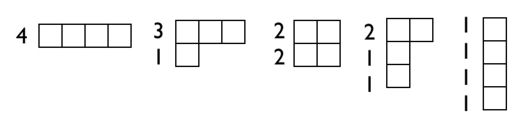
\includegraphics[width=0.6\linewidth]{Immagini/partitions of 4.png}
    \caption{Young diagrams corresponding to the partitions of four.}
    \label{fig: Young diagrams of the partitions of four}
\end{figure}

Permutations reorder the elements of a set $X$ with distinct elements. If one represents the elements of $X$ as letters of the alphabet and each ordering as a word, then each permutation is called an anagram. 
\begin{defn}[multiset]
    A multiset is defined as a set where an element $x_i$ can appear multiple times, specified by its multiplicity $m_i$.
\end{defn}
By this definition, the total number of elements of $X$ is $N = \sum_i m_i$. Different words formed by the elements are the different permutations of the multiset. A priori, $N$ elements can be reordered $N!$ times, but there are $m_1!$ to reorder the elements $x_1$, $m_2!$ ways to reorder the elements $x_2$, and so on. So, the total number of distinct re-orderings of the elements of $X$ is 
\begin{equation}
    \binom{N}{m_1,\dots,m_k} \equiv \frac{N!}{m_1!\cdots m_k!},
\end{equation}
where $k$ is the number of distinct elements of $X$ so that $N = \sum_{i=1}^k m_k$ is a partition of $N$. 

\section{Free groups and presentations}
\begin{defn}[free group]
    Let $G$ be a group and $X = {g_1,\dots,g_n}$ a subset of elements of $G$. If every element $g \in G\setminus\{e\}$ can be uniquely written as a product 
    \begin{equation}
        g = g_{j_1}^{i_1}\cdots g_{j_m}^{i_m},
    \end{equation}
    thus of elements $g_{j_k}$ taken only from the set $X$ with exponents $i_k \in \Z \setminus\{0\}$ such that no two adjacent elements are equal, $G$ is said to be a free group and $X$ is a free set of generators of $G$. 
\end{defn}
In analogy of what was said on multisets, the elements of $X$ are called ``letters'', so that an arbitrary product of letters $g = g_{j_1}^{i_1}\cdots g_{j_m}^{i_m}$ is called a ``word'' where $i_k \in \Z$. If the product satisfies the additional conditions of the previous definition, so $i_k \neq 0$ and $g_{j_i} \neq g_{j_{i+1}}$, the word is said to be a ``reduced word''. One can define a constraint called a ``relation'' and denoted with $r$ by setting a reduced word to be equal to the unit element by an equation
\begin{equation}
    r \equiv g_{j_1}^{i_1} \cdots g_{j_m}^{i_m} = e.
\end{equation}
In general, there can be several independent relations $r_i$ with $i \in \N$. 

A definition of a group $G$ now consists of the sets of generators $X = \{g_1,\dots,g_n\}$ and the complete list of independent relations $r_1,\dots,r_n$, so $G$ can be denoted with the notation
\begin{equation}
    G = \mybraket{g_1,\dots,g_n}{r_1,\dots,r_m},
\end{equation}
which is called a ``presentation'' of the group $G$. 
\begin{ex}
    Some examples of groups and their presentations are the followings:
    \begin{enumerate}
        \item Let $X = \{a\}$ and set $r \equiv a^n = e$. With this relation, the set $X$ generates the cyclic group $\Z_n = \{e,a,\dots,a^n\}$, whose representation is $\Z_n = \mybraket{a}{a^n}$. 
        \item The dihedral group $D_4$ is the group of symmetries of a square. Consider the operations $R$ as the rotation by $\pi/2$ and $f$ as the reflection with respect to the vertical axe passing through the midpoints of opposite sides. It is immediate to see the relations $r_1 \equiv R^4$ and $r_2 \equiv f^2$, but a bit less obvious is the relation $r_3 \equiv RfRf$. So, the dihedral group of order four can be denoted as $D_4 = \mybraket{R,f}{R^4,f^2,RfRf}$. More in general, the dihedral group $D_n$ describes the symmetries of regular polygons with $n$ sides, and can be denoted with the general presentation $D_n = \mybraket{R,f}{R^n,f^2,RfRf}$.
        \item The Pauli group is a finite group of order 16, consisting of the three Pauli matrices $\sigma^1$, $\sigma^2$, $\sigma^3$ and the identity matrix $\MI$ multiplied by the factors $\pm 1$ and $\pm i$, so $G_1$ is
        \begin{equation}
            G_1 = \{\pm\MI,\pm i\MI,\pm\sigma^1,\pm i\sigma^1,\pm\sigma^2,\pm i\sigma^2,\pm\sigma^3,\pm i\sigma^3\}.
        \end{equation}
        Recalling the relations $(\sigma^a)^2 = \MI$ and $\sigma^a\sigma^b = i\epsilon_{abc}\sigma^c$ the Pauli group can be defined through the presentation 
        \begin{equation}
            G_1 = \mybraket{\sigma^1,\sigma^2,\sigma^3}{(\sigma^a)^2,-i\epsilon_{abc}\sigma^a\sigma^b\sigma^c}.
        \end{equation}
    \end{enumerate}
\end{ex}

\section{Braids}
In general, a braid consists of strands which run forward and can pass under or over each other. In Physics, an important related situation is met when one considers word-lines of point particles moving in two dimensional spaces. The particle word-lines then form strands that become entangled, just like knitting strands. This phenomenon gives rise to exotic quantum statistics for quantum particles in two dimension\footnote{The reason why this is not true in three or more space dimension is that there the strands can be untangled} called ``anyons'', which are quasi-particles generalisation of fermions and bosons in three dimension. Here the convention is that the braid is drawn upright with braiding strands beginning from the top and proceeding downwards, the exact opposite of what shown in figure \ref{fig: anyons}. One can imagine that strands are like pieces of string and thus can be moved and deformed continuously. 
\begin{figure}[h]
    \centering
    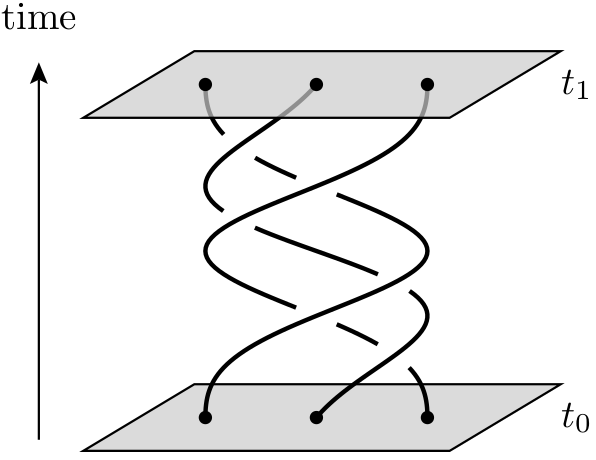
\includegraphics[width=0.4\linewidth]{Immagini/anyons.png}
    \caption{wordlines of three particles moving on a two dimensional plane.}
    \label{fig: anyons}
\end{figure}

In a braid of $n$ strands, the strands can be labelled by an index $i = 1,\dots,n$ running from left to right. A possible way to move strands in a braid is known as the ``Reidermeister move of the second type''\footnote{There exists also the Reidermeister move of the first type which is simply defined as untwisting a strand passing over itself.}, as shown in figure \ref{fig: RM of the II type}. 
\begin{figure}[h]
    \centering
    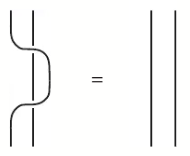
\includegraphics[width=0.3\linewidth]{Immagini/RM of the II type.png}
    \caption{the Reidermeister move of the second type.}
    \label{fig: RM of the II type}
\end{figure}

To form braids, another important basic operation, denoted as $\sigma_i$, consists in the moving of the $i$th strand over the $(i+1)$th strand, as shown in figure \ref{fig: sigma_i and sigma_i^-1 operations}. The inverse operation $\sigma_i^{-1}$ moves the $(i+1)$th strand over the $i$th strand, as shown again in picture \ref{fig: sigma_i and sigma_i^-1 operations}. A crucial rule to note is that after every operation, the strands are indexed again from left to right from 1 to $n$, and next operation is performed one the strands labelled according to the new indexing.
\begin{figure}[h]
    \centering
    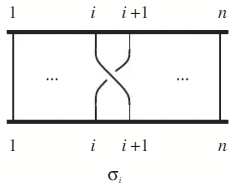
\includegraphics[width=0.35\linewidth]{Immagini/sigma_i operation.png}
    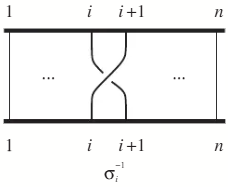
\includegraphics[width=0.335\linewidth]{Immagini/sigma_i^-1 operation.png}
    \caption{the basic operation. (i) $\sigma_i$ which moves $i$th over the $(i + 1)$th strand; (ii) $\sigma_i^{-1}$ which moves $(i + 1)$th over the $i$th strand.}
    \label{fig: sigma_i and sigma_i^-1 operations}
\end{figure}
To illustrate the indexing, consider the sequences of operations $\sigma_i\sigma_i^{-1}$ and $\sigma_i^2 = \sigma_i\sigma_i$. For the first one, after $\sigma_i$, the $i$th strand becomes the $(i+1)$th, and vice versa. With the new indexing, the next operation $\sigma_i^{-1}$ then acts in the opposite way of the first operation, the final result for $\sigma_i\sigma_i^{-1}$ coincides with the initial state, as shown in figure \ref{fig: sigma_i x sigma_i^-1 operation}, so the operation reduces to the trivial one $e$. The same thing happens for $\sigma_i^{-1}\sigma_i$. 
\begin{figure}[h]
    \centering
    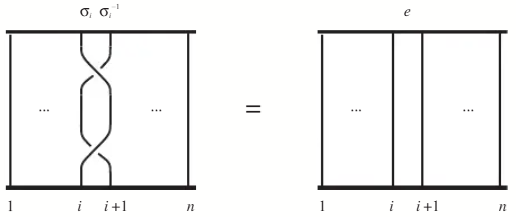
\includegraphics[width=0.7\linewidth]{Immagini/sigma_i x sigma_i^-1 operation.png}
    \caption{equivalence between the identity element $e$ and the sequence of operations $\sigma_i\sigma_i^{-1}$.}
    \label{fig: sigma_i x sigma_i^-1 operation}
\end{figure}

By the same rules, the operation $\sigma_i\sigma_i$ does not reduce to $e$, instead the strands become tangled with a non-trivial final result, as shown in figure \ref{fig: sigma_i^2 operation}. 
\begin{figure}[h]
    \centering
    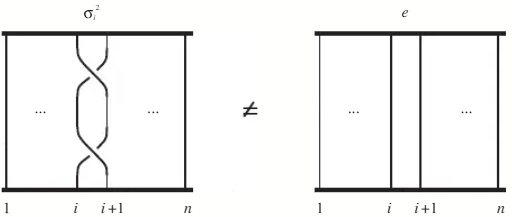
\includegraphics[width=0.7\linewidth]{Immagini/sigma_i^2 operation.png}
    \caption{inequivalence between the identity element $e$ and the sequence of operations $\sigma_i^2$.}
    \label{fig: sigma_i^2 operation}
\end{figure}

After these examples, one can generalise the discussion by moving to more general constructions. For a braid of $n$ strands, the basic operations $\sigma_1,\dots,\sigma_{n-1}$, that can be thought of as the letters of a set $X_{n-1}$, thus, each word is
\begin{equation}
\label{eq: definition of a generic braid}
     \sigma = \sigma_{j_1}^{i_1}\cdots\sigma_{j_m}^{i_m},\quad i_m \in \Z,
\end{equation}
represents a braid. As before, when drawing the braid, one starts from the top, reads the letters of the word from left to right and performs the corresponding operation on the strands, continuing the drawing downwards. The inverse of a generic braid defined in \eqref{eq: definition of a generic braid} is obtained as the product of the inverse operations in the opposite order
\begin{equation}
    \sigma^{-1} = \sigma_{j_m}^{-im}\cdots \sigma_{j_1}^{-i_1}.
\end{equation}
The group generated by $X_{n-1}$ for $n > 2$ is not a free group. There are relations among the generators, because one can move and deform the strands continuously. One relation is due to the fact that the operations of braiding strands that are sufficiently apart from each other are independent operations, so their generators commute
\begin{equation}
\label{eq: commutation relation between braid generators}
    \sigma_i\sigma_j = \sigma_j\sigma_i,\quad |i - j| \ge 2.
\end{equation}
A less obvious relation is the Reidermeister move of the third type
\begin{equation}
\label{eq: Reidermeister move of the III type}
    \sigma_i\sigma_{i+1}\sigma_i = \sigma_{i+1}\sigma_i\sigma_{i+1}.
\end{equation}
It turns out that the diagram in figure \ref{fig: Yang-Baxter relation} also appears in the context of exactly solvable problems in statistical mechanics and quantum field theories, where it is related to a Yang-Baxter relation. This is not an accident, since the conditions that determine the integrability of those models have a connection with the properties of braids. 
\begin{figure}[h]
    \centering
    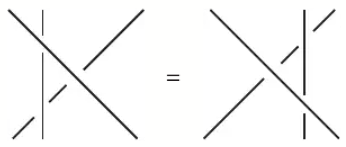
\includegraphics[width=0.4\linewidth]{Immagini/Yang-Baxter relation.png}
    \caption{diagram showing the equivalence $\sigma_i\sigma_{i + 1}\sigma_i = \sigma_{i + 1}\sigma_i\sigma_{i + 1}$, namely the Reidermeister move of the third type.}
    \label{fig: Yang-Baxter relation}
\end{figure}

One can show that the relations \eqref{eq: commutation relation between braid generators} and \eqref{eq: Reidermeister move of the III type} are the only relations between the generators $\sigma_i$. This leads up to define the braid group of $n$ strands $B_n$ by its presentation
\begin{equation}
    B_n = \mybraket{\sigma_1,\dots,\sigma_n}{\sigma_i\sigma_j = \sigma_j\sigma_i,\,\sigma_i\sigma_{i+1}\sigma_i = \sigma_{i+1}\sigma_i\sigma_{i+1}},
\end{equation}
where $|i - j| \ge 2$ in the first relation and $1 \le i \le n - 2$ in the second one. In conclusion, some properties of braid groups are the following:
\begin{enumerate}
    \item $B_1$ is the trivial group $\Z_1 = \{e\}$;
    \item $B_2 \simeq (\Z_2,+)$ so it is an Abelian group;
    \item $B_3$ is non-Abelian;
    \item the braid groups form a nested sequence of subgroups $B_n \subset B_{n + 1}$ for every positive real natural number $n$.
\end{enumerate}

\section{Continuous groups}
Continuous groups are groups having an infinite and uncountable number of elements. Since the order of a continuous group is not a meaningful concept, the ``size'' of a continuous group is instead characterized in terms of its dimension.
\begin{defn}[dimension]
    The dimension of a continuos group $G$ denoted with $\dim{G}$ is the minimum number of real parameters needed to uniquely identify its elements.
\end{defn}
The real parameters identifying an element of a continuos group are called its ``coordinates'', where each one may take values within the whole $\R$, or within a real interval. The definition of a group dimension is distinct from, and more general, the definition of dimension of a vector space. Indeed, continuous groups may, but not necessarily have to, be realized in terms of linear vector spaces. As will discussed later, given the product of two elements $g \cdot g' = g''$, where $g,g' \in G$, the coordinates of $g''$ must be continuous functions of the coordinates $g$ and $g'$. This means that the set of coordinates parametrizing a group form a manifold, called the ``group manifold''. The most interesting continuous groups are Lie groups.
\begin{defn}[Lie group]
    A Lie group is a continuous group whose group manifold is differentiable, so it is possible to take smooth derivatives of the group elements with respect to the coordinates.
\end{defn}
Particularly interesting Lie groups are those defined from certain sets of matrices, with the usual matrix multiplication law as the group composition operation.
\paragraph{$\bm{GL(n,\R)}$ group.} The group of general linear transformations with real coefficients denoted as $GL(n, \R)$ is defined as the subset of matrices in $\R^{n,n}$ having a non-vanishing determinant, with the matrix product as the group multiplication:
    \begin{equation}
        GL(n, \R) = \{ A \in \R^{n,n} : \det A \neq 0 \}.
    \end{equation}
    The identity matrix of size $n \times n$ is the unit element of the group, and the existence of the inverse of any element of $GL(n, \R)$ is guaranteed by the condition that the determinant is different from zero. Note that the determinant of a matrix is a continuous function of its entries. The dimension of $GL(n, \R)$ is $\dim GL(n, \R) = n^2$, like that of $\R^{n,n}$. Note that the constraint that the determinant of the elements of $GL(n, \R)$ is different from zero does not reduce the number of independent real parameters of $GL(n, \R)$. While $GL(n, \R)$ and $\R^{n,n}$ have the same dimension, their group manifolds have a different global structure. In particular, in contrast to $\R^{n,n}$, for which the matrix entries are a set of suitable coordinates, in $GL(n, \R)$ the condition $\det A \neq 0$ for a generic group element $A$ implies that the coordinates parametrizing the group elements cannot take arbitrary values in $\R^{n,n}$, but rather in $\R^{n,n}$ with the exclusion of the hypersurface on which the matrix determinant vanishes (this hypersurface is a set of measure zero in $\R^{n,n}$). Thus the group manifold of $GL(n, \R)$ is divided into two disconnected components (in which the determinant of a generic element is either positive or negative).

\paragraph{$\bm{GL(n,\C)}$ group.} The group of general linear transformations can be generalized, by allowing the matrix elements to take values in the complex field; this leads to the group
    \begin{equation}
        GL(n, \mathbb{C}) = \{ A \in\C^{n,n}) : \det A \neq 0 \},
    \end{equation}
    again with matrix product as the group multiplication. As for the group $GL(n, \R)$, the unit element is the identity matrix of size $n \times n$, and the existence of the inverse of any element of the group is guaranteed by the fact that the determinant is non-vanishing. Since each of the $n^2$ entries of a generic matrix $A \in GL(n, \mathbb{C})$ is a complex number, which can be parametrized by two real coordinates, and since the $\det A \neq 0$ constraint does not reduce the number of independent parameters, the dimension of $GL(n, \mathbb{C})$ is $2n^2$. Finally, note that $GL(n, \R)$ is a proper subgroup of $GL(n, \mathbb{C})$. The group $GL(n, \mathbb{C})$ and its subgroups are called matrix Lie groups.

\paragraph{$\bm{SL(n,\R)}$ group.} The set of special linear transformations of degree $n$ with real coefficients is denoted as $SL(n, \R)$ and is defined as
    \begin{equation}
        SL(n, \R) = \{ A \in \R^{n,n} : \det A = 1 \}.
    \end{equation}
    Note that, since $\det A = 1$ is a special case of $\det A \neq 0$, $SL(n, \R)$ is a subset of $GL(n, \R)$. Taking the matrix product as the composition law, and observing that the product of two matrices with determinant $1$ also has determinant $1$, that the inverse of any matrix of determinant $1$ also has determinant $1$, and that the determinant of the identity matrix is $1$, too, it follows that $SL(n, \R)$ is a proper subgroup of $GL(n, \R)$. The dimension of $SL(n, \R)$ is $n^2 - 1$: the condition that the determinant of each element equals $1$ is expressed as an equation, that reduces the number of independent coordinates from $n^2$ down to $n^2 - 1$.

\paragraph{$\bm{O(n,\R)}$ group.} The orthogonal group of degree $n$ is defined as the group of real matrices (orthogonal matrices) whose inverse coincides with their transpose. For a given matrix $A$, the latter is defined as the matrix obtained from $A$ by interchanging its rows with its columns, $(A^T)_{ab} = A_{ba}$:
    \begin{equation}
        O(n, \R) = \{ A \in GL(n, \R) : A^T A = A A^T = \MI \},
    \end{equation}
    where $\MI$ is the identity matrix of size $n \times n$. It is easy to prove that $O(n, \R)$ (with the matrix product as the group multiplication) is a proper subgroup of $GL(n, \R)$, since:
    \begin{enumerate}
        \item the product of two elements of $O(n, \R)$, $A$ and $B$, is also an orthogonal matrix:
        \begin{equation}
            (AB)^T (AB) = B^T A^T A B = B^T B = \MI;
        \end{equation}
        \item the unit element for the matrix product is the identity matrix, which is an orthogonal matrix $(\MI^T \MI = \MI)$;
        \item the inverse of a generic orthogonal matrix $A$ is also orthogonal:
        \begin{equation}
            (A^{-1})^T A^{-1} = (A A^T)^{-1} = \MI^{-1} = \MI.
        \end{equation}
    \end{enumerate}
    Orthogonal matrices can be seen as linear transformations acting on the $n$-dimensional real vector space $\R^n$ and preserve the modulus of vectors in $\R^n$. Indeed, the modulus of a vector $\vv \in \R^n$ is given by $\sqrt{\sum_{a=1}^n v_a^2} = \sqrt{\vv^T \vv}$. Upon a transformation $A \in O(n, \R)$, the vector $\vv$ gets mapped to $A\vv$, whose modulus is $\sqrt{(A\vv)^T (A\vv)} = \sqrt{\vv^T A^T A \vv} = \sqrt{\vv^T \vv}$, namely it is left invariant. As a consequence, the orthogonal group can be interpreted as a group of rotations and reflections in $\R^n$. To determine the dimension of $O(n, \R)$, note that each element is expressed by a matrix with $n^2$ real entries, but they are not all independent, because the orthogonality condition restricts the number of independent coordinates. In particular, the requirement that $A^T A = \MI$ implies that each diagonal entry of $A^T A$ must be equal to $1$; this imposes $n$ equations. In addition, all of the entries above the diagonal must vanish, and this gives further $n(n-1)/2$ independent equations. If the entries above the diagonal vanish, then so do those below the diagonal, because $A^T A$ is a symmetric matrix. The constraints imposed by the $A A^T = \MI$ condition equivalent. Hence, the orthogonality constraint reduces the number of independent real parameters down to $n^2 - n - n(n-1)/2 = n(n-1)/2$. Finally, note that the orthogonality condition (and the fact that the determinant of a matrix and that of its transpose are equal) also implies that the determinant of any element of $O(n, \R)$ is either $1$ or $-1$, because $\det(A^T A) = \det \MI$ implies $(\det A)^2 = 1$, hence $\det A = \pm 1$. The subset of $O(n, \R)$ including the matrices of determinant $1$ is the special orthogonal group of degree $n$:
    \begin{equation}
        SO(n, \R) = \{ A \in GL(n, \R) : A^T A = A A^T = \MI,\ \det A = 1 \}.
    \end{equation}
    The special orthogonal group of degree $n$ is a proper subgroup of $O(n, \R)$ and its dimension is $\dim SO(n, \R) = n(n-1)/2$, like $O(n, \R)$ (because the determinant of elements of $O(n, \R)$ can only take values $\pm 1$, hence the condition that the determinant equals $1$ for $SO(n, \R)$ elements does not reduce the number of independent real coordinates). $SO(n, \R)$ can be interpreted as the subgroup of $O(n, \R)$ which preserves the orientation of a basis of vectors in $\R^n$. So, for example, acting with a matrix of $SO(3, \R)$ on the vectors of a right-handed orthonormal basis of $\R^3$ results into a rotated basis of vectors, which is still right-handed. Note that, by contrast, the subset of $O(n, \R)$ including the matrices with determinant $-1$ is not a subgroup (in fact, it is not even a magma, since $\det A = \det B = -1$ implies $\det(AB) = 1$). Often the orthogonal groups and their special subgroups are denoted as $O(n)$ and $SO(n)$.

\paragraph{$\bm{U(n)}$ group.} The generalization of the orthogonal group of degree $n$ to the complex field is the unitary group of degree $n$, defined as
    \begin{equation}
        U(n) = \{ A \in GL(n, \C) : A^\dg A = A A^\dg = \MI \},
    \end{equation}
    where $A^\dg = (A^*)^T = (A^T)^*$ is the conjugate transpose of $A$: $(A^\dg)_{ij} = (A_{ji})^*,$ with $*$ denoting complex conjugation. Note that $(AB)^\dg = B^\dg A^\dg$. These matrices preserve the modulus of complex vectors $\vv \in \C^n$, defined as $\sqrt{\sum_{a=1}^n z_a^* z_a} = \sqrt{\vv^\dg \vv}$. A generic element $A \in U(n)$ maps a vector $\vv$ to $A\vv$, whose modulus is $\sqrt{(A\vv)^\dg (A\vv)} = \sqrt{\vv^\dg A^\dg A \vv} = \sqrt{\vv^\dg \vv}$, namely is left invariant by the action of $A$. Hence unitary matrices can be interpreted as ``rotations'' in $\C^n$. (More generally, a linear map $A : V \to W$ between two vector spaces $V$ and $W$ that preserves the lengths of vectors is called an isometry.) $U(n)$ is a proper subgroup of $GL(n, \C)$. One can show that $\dim U(n) = n^2$: Starting from the dimension of $GL(n, \C)$, which is $2n^2$ (where the factor $2$ accounts for the fact that each matrix element has a real and an imaginary part), the dimension of $U(n)$ can be obtained by subtracting from it the number of independent constraints that the $U(n)$ matrix entries must obey. From the requirement that $A^\dg A = \MI$ follows, first of all, that each diagonal element of $A^\dg A$ must be equal to $1$:
    \begin{equation}
    \label{eq: unitarity condition of U(n) group I}
        (A^\dg A)_{ii} = \sum_{k=1}^n A^\dg_{ik} A_{ki} = (\MI)_{ii} = \delta_{ii} = 1, \quad \forall i : 1 \le i \le n.
    \end{equation}
    Using the fact that $A^\dg_{ik} = A^*_{ki}$, \eqref{eq: unitarity condition of U(n) group I} can be rewritten as
    \begin{equation}
    \label{eq: unitarity condition of U(n) group II}
        \sum_{k=1}^n A^*_{ki} A_{ki} = \sum_{k=1}^n |A_{ki}|^2 = 1, \quad \forall i : 1 \le i \le n.
    \end{equation}
    Equation \eqref{eq: unitarity condition of U(n) group II} corresponds to $n$ constraints (not $2n$, because a sum of squared moduli of complex numbers is necessarily a real, non-negative number, namely the imaginary part of each sum is already necessarily zero, without imposing any constraint on it). Conversely, for the $n(n-1)/2$ elements above the diagonal of the $A^\dg A$ matrix, the conditions
    \begin{equation}
    \label{eq: above diagonal elements condition of U(n) group}
        (A^\dg A)_{ij} = \sum_{k=1}^{n} A_{ik}^\dg A_{kj} = 0, \quad 1 \le i < j \le n,
    \end{equation}
    enforce the vanishing of the real and of the imaginary part, and thus correspond to two independent constraints for each element. Finally, the constraints on the remaining $n(n-1)/2$ elements below the diagonal of the $A^\dg A$ turn out to be equivalent to those expressed by \eqref{eq: above diagonal elements condition of U(n) group}. Also, one can check that the same constraints arise if one requires $A A^\dg = \MI_n$. To conclude, note that the dimension of the unitary group of degree $n$ is given by $\dim U(n) = 2n^2 - n - 2\, n(n-1)/2 = n^2$. Note that, according to the definition \eqref{eq: unitarity condition of U(n) group I}, $U(1) = \{ a \in \C : a^* a = 1 \}$, so the group manifold of $U(1)$ can be identified with the circle of unit radius on the complex plane. The subset of $U(n)$ containing matrices of determinant equal to $1$ constitutes the special unitary group of degree $n$:
    \begin{equation}
        SU(n) = \{ A \in U(n), \det A = 1 \}.
    \end{equation}
    This is a proper subgroup of $U(n)$, and its dimension can be computed by noting that, in addition to the constraints that every $U(n)$ matrix must satisfy, the requirement $\det A = 1$ imposes one additional condition (not two, because from $A^\dg A = \MI_n$, which holds for every unitary matrix $A$, and from the property that $\det A^\dg = (\det A)^*$, already follows that $\det(A^\dg A) = \det(A^\dg)\det A = (\det A)^* \det A = |\det A|^2 = \det \MI_n = 1$, namely the real and imaginary parts of $\det A$ cannot be arbitrary numbers, since they already satisfy the constraint that $|\det A| = 1$). Thus $\dim SU(n) = (\dim U(n)) - 1 = n^2 - 1$. The subset of $\R^{2n,2n}$ containing the matrices $M$, called ``symplectic matrices,'' that satisfy the property
    \begin{equation}
        M^T \Omega M = \Omega, \quad \Omega =
        \begin{pmatrix}
        0_n & \MI_n \\
        -\MI_n & 0_n
        \end{pmatrix}.
    \end{equation}

\section{Groups acting on a set}
\begin{defn}[left-action]
    Given a group $G$ and a set $X$, a left-action of $G$ on $X$ is a homomorphism
    \begin{equation}
        L : G \to \Perm{X},\quad g \mapsto L_g.
    \end{equation}
\end{defn}
Since a left-action is a group homomorphism, it preserves the group multiplication 
\begin{equation}
    \forall g_1,g_2 \in G,\,\forall x \in X : L_{g_2}(L_{g_1}(x)) = L_{g_2 \cdot g_1}(x).
\end{equation}
\begin{defn}[left group-space]
    Given a group $G$, a set $X$ is called a left group-space of $G$, or a left $G$-space, if there exists a left-action of $G$ on $X$.
\end{defn}
Similarly, one can define a right-action and a right group-space.
\begin{defn}[right-action]
    Given a group $G$ and a set $X$, a right-action of $G$ on $X$ is a homomorphism
    \begin{equation}
        R : G \to \Perm{X},\quad g \mapsto R_g,
    \end{equation}
    such that it preserves the group multiplication
    \begin{equation}
        \forall g_1,g_2 \in G,\,\forall x \in X : R_{g_2}(R_{g_1}(x)) = R_{g_2 \cdot g_1}(x).
    \end{equation}
\end{defn}
\begin{defn}[right group-space]
    Given a group $G$, a set $X$ is called a right group-space of $G$, or a right $G$-space, if there exists a right-action of $G$ on $X$.
\end{defn}
Given a group $G$, two left $G$-spaces $X$ and $X'$ can be identified, if there is a bijection $i : X \to X'$ such that, for any $g \in G$ and for any $x \in X$, one has $i(L_g(x)) = L_g'(i(x))$, where $L$ and $L'$ are the left-actions of $G$ on $X$ and on $X'$, respectively. An analogous definition can be made for right $G$-spaces and right-actions. 
\begin{defn}[orbit]
    Given a left $G$-space $X$ of a group $G$, the orbit of a point $x \in X$ under the left-action $L$ of $G$ on $X$ is the set
    \begin{equation}
        O_x = \{g \in G\ : L_g(x) \}.
    \end{equation}
\end{defn}
In other words, the orbit of a point $x \in X$ is the subset of $X$ containing all points that can be reached from $x$ by acting on it with the left-action of some element of $G$. Given a group $G$, a left-action of $G$ on $X$ is said to be ``transitive'' when all elements of $X$ belong to the same orbit, in other words $X/G$ contains only one element. In practice, a left-action $L$ of a group $G$ on a set $X$ is transitive when for any $x \in X$ and any $y \in Y$, there exists an element $g \in G$, such that $y = L_g(x)$, so a left-action is transitive if it connects evey pair of elements in $X$. 
\begin{defn}[homogeneous space]
    A set $X$ is said to be a homogeneous space under the action of $G$, when the action of $G$ on $X$ is transitive.
\end{defn}
\begin{ex}
    Let $G = \Z_2 = \{e,a\}$ and $X = \R$. Consider the left-action $L$ such that $L_e(x) = x$ and $L_a(x) = -x$. The orbit of a generic point $x \in X$ contains either two distinct elements $O_x = \{x,-x\}$ if $x \neq 0$ or just $x$ itself if $x = 0$. Hence, two generic elements $x,y \in X$ belong to the same orbit only if $x = \pm y$. The action is not transitive, because $X/G$ contains infinitely many orbits, namely one for each non-negative real number.
\end{ex}
\begin{defn}[isotropy group]
    Given a group $G$, a left $G$-space $X$, and an element $x \in X$, the isotropy group of $x$ is the subgroup of $G$ containing all elements that leave $x$ invariant
    \begin{equation}
        G_x = \{g \in G : L_g(x) = x\}.
    \end{equation}
\end{defn}
For some points $x$ it may turn out that $G_x = G$, so $L_g(x) = x$ for any $g \in G$; in this case $x$ is said to be a ``fixed point'' under the action of $G$. One can also be interested in the converse problem, that of finding all the points that are left invariant by the action of a given element $g$ of a group $G$. 
\begin{defn}[isotropy set]
    Let $g$ be an element of a group $G$ acting on a set $X$, the set of points left invariant by the left-action of $g$ is defined as
    \begin{equation}
        X^g = \{x \in X : L_g(x) = x\}.
    \end{equation}
\end{defn}
Note that for the unit element $e$ one have $X^e = X$ since $e$ is always represented by the identity map. A particularly interesting case of group-space is the group itself $X = G$. The simplest left and right-actions are simply the ``translations'', so the actions defined by multiplication by a group element on the left and on the right. The left translation of a group $G$ is the group homomorphism $L : G \to \Perm{G}$, with $g \mapsto L_g$, defined $L_g(g') = g\cdot g'$ for any $g' \in G$. Similarly, the right translation is the group homomorphism $R : G \to \Perm{G}$, with $g \mapsto R_g$, defined as $R_g(g') = g'\cdot g$ for any $g' \in G$. Note that the left, or right, translation is always a transitive action: every group element belongs to the orbit of the unit element $e$, since $L_g(e) = g \cdot e = g$, or $R_g(e) = e \cdot g = g$, in other words $O_e = G$. A more interesting way to define the group action on itself is by conjugation.
\begin{defn}[conjugation]
    The conjugation of a group $G$ is the group homomorphism $L : G \to \Perm{G}$, with $g \mapsto L_g$, defined as
    \begin{equation}
        L_g(g') = g\cdot g' \cdot g^{-1},\quad \forall g' \in G.
    \end{equation}
\end{defn}
\begin{defn}[conjugacy class]
    A conjugacy class of an element of a group $G$ is defined as its orbit under conjugation.
\end{defn}
In other words, the conjugacy class of a generic element $g \in G$ is the subset of $G$ containing all elements $g$ that can be written in the form $g' = x \cdot g \cdot x^{-1}$ for some $x \in G$. Then $g$ and $g'$ are said to be ``conjugate'', and $x$ is called the ``conjugating element''. In general, conjugation is not a transitive action. It is also interesting to consider the action of a subgroup $H \subset G$ on $G$. In particular, the right-action of $H$ on $G$ defined by translation, $R_h(g) = g \cdot h$, is not necessarily transitive if $H$ is a proper subgroup. 
\begin{defn}[left coset]
    Given a group $G$ and a subgroup $H \subset G$, the left coset associated with an element $g \in G$ is the orbit of $g$ under right translation by elements of $H$, so the set 
    \begin{equation}
        gH = \{g' \in G : \exists h \in H : g' = g \cdot h\}.
    \end{equation}
\end{defn}
\begin{defn}[right coset]
    Given a group $G$ and a subgroup $H \subset G$, the right coset associated with an element $g \in G$ is the orbit of $g$ under left translation by elements of $H$, so the set 
    \begin{equation}
        Hg = \{g' \in G : \exists h \in H : g' = h \cdot g\}.
    \end{equation}
\end{defn}
The set of left cosets forms the quotient space $G/H = \{gH : g \in G\}$, while the set of right cosets forms the quotient space $H\setminus G = \{Hg : g \in G\}$. Obviously, when $G$ is an Abelian, left and the right cosets coincide. Note that, if two elements $g,g' \in G$ can be obtained from each other via right translation by an element of the subgroup, so $g' = g\cdot h$ with $h \in H$, then their left and right cosets coincide $gH = Hg$. The inverse is also true: if the left cosets of two elements $g,g'\in G$ coincide, the $g^{-1}\cdot g' \in H$, so it exists a unique $h \in H$ such that $g' = g\cdot h$. Finally, one can prove that the elements of each coset can be put in a one-to-one correspondence with the elements of $H$ itself. 
\begin{proof}
    For a given $g \in G$, the mapping $f_g : H \to gH$, with $h \mapsto g\cdot h$, is surjective, by definition of $gH$. It also is injective, because multiplying $g\cdot h_1 = g\cdot h_2$ by $g^{-1}$ on the left if follows that $h_1 = h_2$. Thus, $f_g$ is a bijection, so it is a one-to-one correspondence between $H$ and the generic coset $gH$.
\end{proof}
In particular, if $H$ is a finite subgroup, then the order of all cosets must equal $|H|$. This leads to the following theorem. 
\begin{teo}[Lagrange's theorem]
\label{teo: Lagrange's theorem}
    The order $|H|$ of any subgroup $H$ of a finite group $G$ must be a divisor of $|G|$.
\end{teo}
\begin{proof}
    Under the right-action of $H$, the group $G$ is partitioned into mutually disjoint orbits $gH$, each having the same order as $H$. Hence, $|G| = n|H|$ for some $n \in \N$.
\end{proof}
\begin{corl}
    If $p$ is a prime number, then $\Z_p$ is the only subgroup of order $p$.
\end{corl}
\begin{proof}
    Consider a generic finite group $G$ of order $p$, and let $g$ be an element of $G$ different from the unit element $e$ of $G$. Let $m$ denote the order of $g$; since $g \neq e$, it follows that $m > 1$. Then $H = \{e,g,\dots,g^{m - 1}\} \simeq \Z_m$ is a subgroup of $G$. Lagrange's theorem implies $p = nm$, but since $p$ is prime and $m  > 1$, then necessarily $n = 1$ and $p = m$, thus $|G| = |H|$. Then $G$ coincides with $H$, which is isomorphic to $\Z_p$. Thus any finite group of order $p$ is isomorphic to $Z_p$, which is the only abstract group of order $p$.
\end{proof}
Note that the quotient space $G/H$ is a $G$-space, if one defines the left-action $L : G \to \Perm{G/H}$, with $g \mapsto L_g$, as
\begin{equation}
    L_g(g'H) = gg'H.
\end{equation}
Note that any two arbitrary elements of $G/H$ always belong to the same orbit defined by $L$, because $y = g_2g_1^{-1} \in G$, and $L_yg_1H = g_2g_1^{-1}g_1H = g_2H$, thus the action is transitive. The inverse statement is also true.
\begin{teo}
\label{teo: correspondence quotient-set}
    Every group $G$ acting transitively on a set $X$ admits a subgroup $H$, such that the quotient space $G/H$ is in one-to-one correspondence with $X$.
\end{teo}
\begin{proof}
    For a given $x \in X$, consider its isotropy group $G_x$ as a subgroup $H$. Consider the map $i : G/H \to X$ defined as $i(gH) = L_g(x)$. Note that $i$ is well defined, so $i(gH)$ does not depend on the representative $(g)$ chosen in $gH$, because the definition of $gH$ implies that for any other representative $g' \in gH$ there exists ah $h \in H$ such that $g = g'h$. Thus $L_g(x) = L_{g'h}(x)$, and, since $L$ is a group homomorphism, this implies $L_g(x) = L_{g'}(L_h(x)$. But $L_h(x) = x$, because $h \in H$ and $H$ is the isotropy group of $x$. As a consequence, $L_g(x) = L_{g'}(x)$. Moreover, $i$ is injective, because $i(gH) = i(g'H)$ means $L_g(x) = L_{g'}(x)$, which implies $x = L_{g^{-1}g'}(x)$, which means that $L_{g^{-1}g'}$ leaves $x$ invariant, so $g^{-1}g' \in H$. This means that $g' = gh$, thus the cosets $gH$ and $g'H$ are equal. Finally, $i$ is also surjective; since $G$ acts transitively, for any $x' \in X$ there exists a $g \in G$ such that $x' = L_g(x)$. But the right-hand side of the latter equation equals $i(gH)$, hence for any $x' \in X$ there exists a $g \in G$ such that $x' = i(gH)$.Thus there exists a bijective correspondence $i$ between $X$ and $G/H$. 
\end{proof}
\begin{corl}
\label{corl: correspondence quotient-set}
    The orbit of a point $x \in X$ can be identified with $G/G_x$.
\end{corl}
\begin{proof}
    Since $G$ acts transitively on its orbit, the statement of the corollary is a consequence of the previous theorem.
\end{proof}
Thus the orbits are determined by the subgroups of $G$; in other words, the action of $G$ on $X$ is determined by its subgroup structure.
\begin{ex}
    Consider the left-action of $G = SO(3,\R)$ on $\R^3$. The orbits are the spheres $|x^2| = x_1^2 + x_2^2 + x_3^2 = r^2$, which can be identified with the $S^2$ sphere for any $r > 0$. Given the point $x = (0,0,r)$ on each orbit $r > 0$, its isotropy group is
    \begin{equation}
        G_x = \bigg\{
        \begin{pmatrix}
            A_{2 \times 2} & 0 \\
            0 & 1 
        \end{pmatrix} : A_{2 \times 2} \in SO(2,\R)
        \bigg\} \simeq SO(2,\R).
    \end{equation}
    By theorem \ref{teo: correspondence quotient-set} and its corollary \ref{corl: correspondence quotient-set}, it follows that $SO(3,\R)/SO(2,\R) \simeq S^2$.
\end{ex}

If $G$ is a finite group acting on a finite set $X$, by a similar argument as the proof of Lagrange's theorem the following one is derived.
\begin{teo}[orbit stabilizer]
    If $G$ is a finite group acting on a finite set $X$, then it is true that
    \begin{equation}
        |G| = |G_x|\cdot |O_x|,\quad \forall x \in X.   
    \end{equation}
\end{teo}
The following lemma is sometimes useful in combinatorial problems.
\begin{lem}[Burnside's lemma]
    Let $G$ be a finite group acting on a finite set $X$. The number of orbits $|X/G|$ is given by
    \begin{equation}
        |X/G| = \frac{1}{|G|}\sum_{g \in G}|X^g|.
    \end{equation}
\end{lem}
Since the quotient space $G/H$ is constructed out of a group and its subgroup, it is natural to ask if it can also be a group. The first guess for a multiplication law would be $(g_1H)(g_2H) = g_1g_2H$. This definition would be meaningful if the right-hand side were independent of the labelling of the cosets, but this is not always the case; the first factor on the left-hand side is such that $g_1H = g_2H$ for any $h \in H$, so one could replace $g_1$ with $g_1h$; however, on the right-hand side it is not necessarily true that $g_1g_2H$ and $g_1hg_2H$ coincide. To endow $G/H$ with a meaningful group multiplication, it is convenient to require $H$ to be a normal subgroup. If that is the case, then the quotient space $G/H$ can be endowed with group structure by defining the group multiplication as
\begin{equation}
\label{eq: group multiplication of G/H}
    (g_1H)(g_2H) = g_1g_2H,\quad \forall g_1H,g_2H \in G/H.
\end{equation}
The fact that $H$ is a normal subgroup makes the right-hand side uniquely defined, in the sense that it makes the definition of the group multiplication meaningful: on the left-hand side, $g_1$ and $g_2$ are defined only up to right translations by elements of $H$, so that the right-hand side of the equation above could be replaced by $g_1h_1g_2h_2H$. This is obviously equal to $g_1h_1g_2H$, so the ambiguity in the definition of $g_2$ is not a problem. If $H$ is a normal subgroup, then there exists an $h \in H$ such that $h_1g_2 = g_2h$; then $g_1h_1g_2H = g_1g_2hH$ which in turn is equal to $g_1g_2H$, so the right-hand side of \eqref{eq: group multiplication of G/H} is unaffected by the ambiguity in the definition of $g_1$ and $g_2$. It is trivial to show that this definition of group multiplication in $G/H$ satisfies associativity that it admits a unit element and that every element $gH \in G/H$ has $g^{-1}H$ as its inverse. With the multiplication defined by \eqref{eq: group multiplication of G/H}, the quotient space $G/H$ becomes a group called the ``quotient group''. Note that, by Lagrange's theorem \ref{teo: Lagrange's theorem}, if $G$ is a finite group then the order of $G/H$, or of $H \setminus G$, is $|G|/|H|$.
\begin{ex}
    Consider the cyclic group $\Z_{2N} = \{e, a, a^2, \ldots, a^{2N-1}\}$, for a generic $N \in \N_0$ and its subset $H = \{e, a^2, a^4, \ldots, a^{2N-2}\}$. It is easy to prove that $H$ is a subgroup of $\Z_{2N}$. Since cyclic groups are Abelian, $H$ is normal. The two cosets are $eH = a^2H = \cdots = a^{2N-2}H$ and $aH = \{a, a^3, a^5, \ldots, a^{2N-1}\} = a^3H = \cdots = a^{2N-1}H$. Since $(eH)^2 = e^2H = eH$, while $(aH)(eH) = aeH = aH$, $(eH)(aH) = eaH = aH$, and $(aH)^2 = a^2H = eH$, the quotient group $\Z_{2N}/H$ is isomorphic to $\Z_2$.
\end{ex}
\begin{ex}
    Let $G = SU(2)$ and $H = \{\MI_2, -\MI_2\} \simeq \Z_2$. Obviously $A \in SU(2)$ satisfies the property $A(\pm \MI_2) = \pm \MI_2 A$, hence $H$ is a normal subgroup. Thus the quotient space $SU(2)/\Z_2$ is a group; in particular, it turns out to be isomorphic to $SO(3, \R)$.
\end{ex}
\begin{defn}[centre]
    The centre of a group $G$, denoted with $\Z(G)$, is the set of elements that commute with every element of $G$
    \begin{equation}
        \Z(G) := \{z \in G : \forall g \in G,\,z \cdot g = g \cdot z\}.
    \end{equation}
\end{defn}
One can prove that the centre of a group is a subgroup and obviously it is Abelian. By the definition of centre definition, a group $G$ is Abelian if and only if $\Z(G) = G$. Moreover, the centre is also normal; hence, the quotient space $G/\Z(G)$ is always a group. If the centre is trivial $\Z(G) = \{e\}$ then $G/\Z(G) \simeq G$. On the other hand, the centres of some non-Abelian groups are as follows:
\begin{enumerate}
    \item $G = S_3$ has a trivial centre: $\Z(G) = \{e\}$;
    \item $G = D_4$ has centre $\Z(G) = \{e, a^2\} \simeq \Z_2$; the quotient group $G/\Z(G)$ is isomorphic to the Klein four-group $\Z_2 \times \Z_2$;
    \item $G = Q_8$ has centre $\Z(G) = \{e, -e\} \simeq \Z_2$; the quotient group $G/\Z(G)$ is isomorphic to the Klein four-group $Z_2 \times Z_2$;
    \item $G = SO(2k+1, \R)$, with $k \geq 1$, has a trivial centre $\Z(G) = \{e\}$;
    \item $G = SO(2k, \R)$, with $k \geq 2$, has centre $\Z(G) = \{e, -e\} \simeq Z_2$;
    \item $G = U(N)$ has centre $\Z(G) = \{\exp(i\theta),\, \theta \in [0,2\pi)\} \simeq U(1)$;
    \item $G = SU(N)$ has centre $\Z(G) = \{\exp(2k\pi i/N)\,\MI_N,$ for $k \in [0,N-1]\}$, which is isomorphic to $\Z_N$;
    \item $G = Sp(2N, \R)$ has centre $\Z(G) = \Z_2$;
    \item $G = \G_2$ has a trivial centre $\Z(G) = \{e\}$;
    \item $G = \F_4$ has a trivial centre $\Z(G) = \{e\}$;
    \item $G = \E_6$ has centre $\Z(G) = \Z_3$;
    \item $G = \E_7$ has centre $\Z(G) = \Z_2$;
    \item $G = \E_8$ has a trivial centre $\Z(G) = \{e\}$.
\end{enumerate}

There is another way of finding normal subgroups and quotient groups that uses the following definitions.
\begin{defn}[kernel of a group homomorphism]
\label{defn: kernel of a group homomorphism}
    Given two groups $G_1$ and $G_2$ and the group homomorphism $\mu : G_1 \to G_2$, the kernel of $\mu$, denoted as $\ker{\mu}$, is the subgroup of $G_1$ containing the elements mapped to the unit element of $G_2$ by $\mu$, thus is the set
    \begin{equation}
        \ker{\mu} = \{g_1 \in G_1 : \mu(g_1) = e_2 \in G_2\} \subseteq G_1.
    \end{equation}
\end{defn}
\begin{defn}[image of a group homomorphism]
\label{defn: image of a group homomorphism}
    Given two groups $G_1$ and $G_2$ and the group homomorphism $\mu : G_1 \to G_2$, the image of $\mu$, denoted as $\im{\mu}$, is the subgroup of $G_2$ containing the elements that can be obtained by applying $\mu$ to some element of $G_1$, thus is the set
    \begin{equation}
        \im{\mu} = \{g_2 \in G_2 : \exists g_1 \in G_1 : g_2 = \mu(g_1)\} \subseteq G_2.
    \end{equation}
\end{defn}
One can prove that $\ker{\mu}$ is a subgroup of $G_1$ and that $\im{\mu}$ is a subgroup of $G_2$. Moreover, $\ker{\mu}$ is a normal subgroup; in fact, for any $k \in \ker{\mu}$ and for any $g \in G_1$, one has
\begin{equation}
    \mu(gkg^{-1}) = \mu(g)\mu(k)\mu(g^{-1}) = \mu(g)e_2\mu(g^{-1}) = \mu(g)\mu(g^{-1}) = e_2,
\end{equation}
hence $gkg^{-1} \in \ker{\mu}$. Since $\ker{\mu}$ is a normal subgroup of $G_1$, it is possible to define the quotient group $G_1/\ker{\mu}$. This quotient group turns out to be isomorphic to $\im{\mu}$. 
\begin{teo}
\label{teo: G/ker - im isomorphic relation}
    Given two groups $G_1$ and $G_2$ and the group homomorphism $\mu : G_1 \to G_2$, the quotient group $G_1/\ker{\mu}$ is isomorphic to $\im{\mu}$.
\end{teo}
\begin{proof}
    To simplify the notation, let $K$ denote $\ker{\mu}$. Consider the homomorphism 
    \begin{equation}
        i : G_1/K \to \im{\mu},\quad g\mapsto i(gK) = \mu(g).
    \end{equation}
    The definition is meaningful, because if $gK = g'K$ then there is a $k \in K$  such that $g' = gk$, then $i(g'K) = \mu(g') = \mu(gk)$. Since $\mu$ is a group homomorphism, this equals $\mu(g)\mu(j)$, and since $k \in K$ one has $\mu(k) = e_2$, so that $i(g'K) = \mu(g) = i(gK)$, so $i$ is well defined. One can prove that $i$ is injective: $i(gK) = i(g'K)$ means $\mu(g) = \mu(g')$; multiply both sides of this equation by $\mu(g)^{-1}$ one the left, one obtains $e_2 = \mu(g)^{-1}\mu(g')$. Since $\mu$ is a group homomorphism, this implies $e_2 = \mu(g^{-1})\mu(g') = \mu(g^{-1}g')$. This means that $g^{-1}g' \in K$, namely that there exists an element $k \in K$ such that $g' = gk$. This implies that $g'K = gkK = gK$. In addition, $i$ is also surjective. Indeed, $\im{\mu}$ contains all elements of $G_2$ which can be written as $\mu(g)$ for some $g \in G_1$. By definition of $i$, each of these elements is also the image of $gK \in G_1/K$. Being a group homomorphism which is simultaneously injective and surjective, $i$ is a group isomorphism. This implies that $G_1/\ker{\mu}$ is isomorphic to $\im{\mu}$.
\end{proof}
\begin{ex}
    One can show that $SU(2)/\Z_2 \simeq SO(3,\R)$ by constructing a surjective group homomorphism $\mu : SU(2) \to SO(3,\R)$ with the property that $\ker{\mu} = \{\MI_2, -\MI_2\} \simeq \Z_2$. One possible homomorphism is the one mapping a generic $SU(2)$ matrix $A$ to the $SO(3,\R)$ matrix of components
    \begin{equation}
        [\mu(A)]_{ab} = \frac{1}{2}\tr{(\sigma^a A \sigma^b A^{-1})},\quad \forall a,b \in \{1,2,3\},
    \end{equation}
    where $\sigma^a$ and $\sigma^b$ are two of the Pauli matrices. The fact that $\mu$ is a group homomorphism can be proved using the properties of the Pauli matrices. Also, $\mu$ is not injective since
    \begin{equation}
        \begin{split}
            [\mu(-A)]_{ab} &= \frac{1}{2}\tr{[\sigma^a(-A)\sigma^b(-A^{-1})]} \\
            &= \frac{1}{2}\tr{(\sigma^a A \sigma^b A^{-1})} \\
            &= [\mu(A)]_{ab}.
        \end{split}
    \end{equation}
    Furthermore, this implies that $\ker{\mu}  = \{\MI_2, -\MI_2\}$, and from theorem \ref{teo: G/ker - im isomorphic relation} one can conclude that $SU(2)/\Z_2 \simeq SO(3)$.
\end{ex}
